\documentclass{comjnl}

% Package to generate and customize Algorithm as per ACM style
\usepackage[ruled]{algorithm2e}
\usepackage{amsmath}
\usepackage[dvips]{epsfig}
\usepackage{eurosym}         % euro symbol
\usepackage{graphicx}
\usepackage[utf8]{inputenc}  % text encoding
\usepackage{times}
\usepackage{url}

\renewcommand{\algorithmcfname}{ALGORITHM}
\SetAlFnt{\small}
\SetAlCapFnt{\small}
\SetAlCapNameFnt{\small}
\SetAlCapHSkip{0pt}
\IncMargin{-\parindent}

% Document starts
\begin{document}

% Page heads
\markboth{G. Romero et al.}{GPU Parallel Computation in Bioinspired Algorithms. A review}

% Title portion
\title{GPU Parallel Computation in Bioinspired Algorithms. A review}

%\author{G. Romero, M.G. Arenas, P.A. Castillo, A.M. Mora, P. Garcia and J.J. Merelo \affil{University of Granada}}

\author{G. ROMERO \affil{University of Granada}
M.G. ARENAS \affil{University of Granada}
P.A. CASTILLO \affil{University of Granada}
A.M. MORA \affil{University of Granada}
P. GARCIA-SANCHEZ \affil{University of Granada}
J.J. MERELO \affil{University of Granada}}

%Department of Architecture and Computer Technology. CITIC (University of Granada), \email{{gustavo,mgarenas,pedro,amorag,pgarcia,jmerelo}@atc.ugr.es }

%%%%%%%%%%%%%%%%%%%%%%%%%%%%%%%%%%%%%%%%%%%%%%%%%%%%%%%%%%%%%%%%%%%%%%%%%%%%%%%

\begin{abstract}
%Computer algorithms can solve large problems. Run times can be high if their execution require a high amount of computational power. Parallelization is an extended approach for improving time and quality of the solutions. Advances in the gaming industry led to the production of low-cost and high performance graphics processing units (GPUs) which offer more computational resources than traditional central processing units (CPUs). GPUs have arrive to PCs and mobile devices as these units are now included in every one of them. This work presents a review of hardware and software advances in the area of bioinspired methods.

Many problems require high amount of computational power to be addressed, so parallelization of algorithms has been used to improve the time and quality of the solutions. Traditionally these algorithms have been executed in central processing units (CPUs), but the advances in the gaming industry have led to the production of low-cost and high performance graphics processing units (GPUs) included in almost every PC or even in every mobile device. The GPUs (in conjunction with CPUs) can offer more speedup than traditional CPUs, so many researchers are migrating their algorithm to these systems. This work presents a review of hardware and software advances, and their application in the area of bioinspired algorithms. We also propose a taxonomy of classification of the actual parallelization methods in GPUs and a review of the literature in this area.
\end{abstract}

%%%%%%%%%%%%%%%%%%%%%%%%%%%%%%%%%%%%%%%%%%%%%%%%%%%%%%%%%%%%%%%%%%%%%%%%%%%%%%%

\category{I.3.1}{Hardware Architecture}{Graphics processors, Parallel processing}

\terms{GPUs, Parallel Computation, Bioinspired Algorithms, Review}

\keywords{GPUs, Parallel Computation, Bioinspired Algorithms, Review}

\acmformat{G. Romero, M.G. Arenas, P.A. Castillo, A.M. Mora, P. García-Sánchez and J.J. Merelo. 2014. GPU Parallel Computation in Bioinspired Algorithms. A review.}

\begin{bottomstuff}
Author's addresses: Department of Architecture and Computer Technology. CITIC (University of Granada).
\end{bottomstuff}

\maketitle

%%%%%%%%%%%%%%%%%%%%%%%%%%%%%%%%%%%%%%%%%%%%%%%%%%%%%%%%%%%%%%%%%%%%%%%%%%%%%%%
\section{Introduction}
\label{sec:intro}
%%%%%%%%%%%%%%%%%%%%%%%%%%%%%%%%%%%%%%%%%%%%%%%%%%%%%%%%%%%%%%%%%%%%%%%%%%%%%%%

General-purpose computing on graphics processing units (GPGPU) is the technique of using a Graphics Processing Unit (GPU), which typically handles computation only for computer graphics, to perform computation in applications traditionally handled by the central processing unit (CPU). Recently there has been a growing interest in GPU computation. The fact that this kind of processors has the ability to perform restricted parallel processing has elicited considerable interest among researchers with applications that require intensive parallel computation.

\begin{figure}[ht]
\centerline{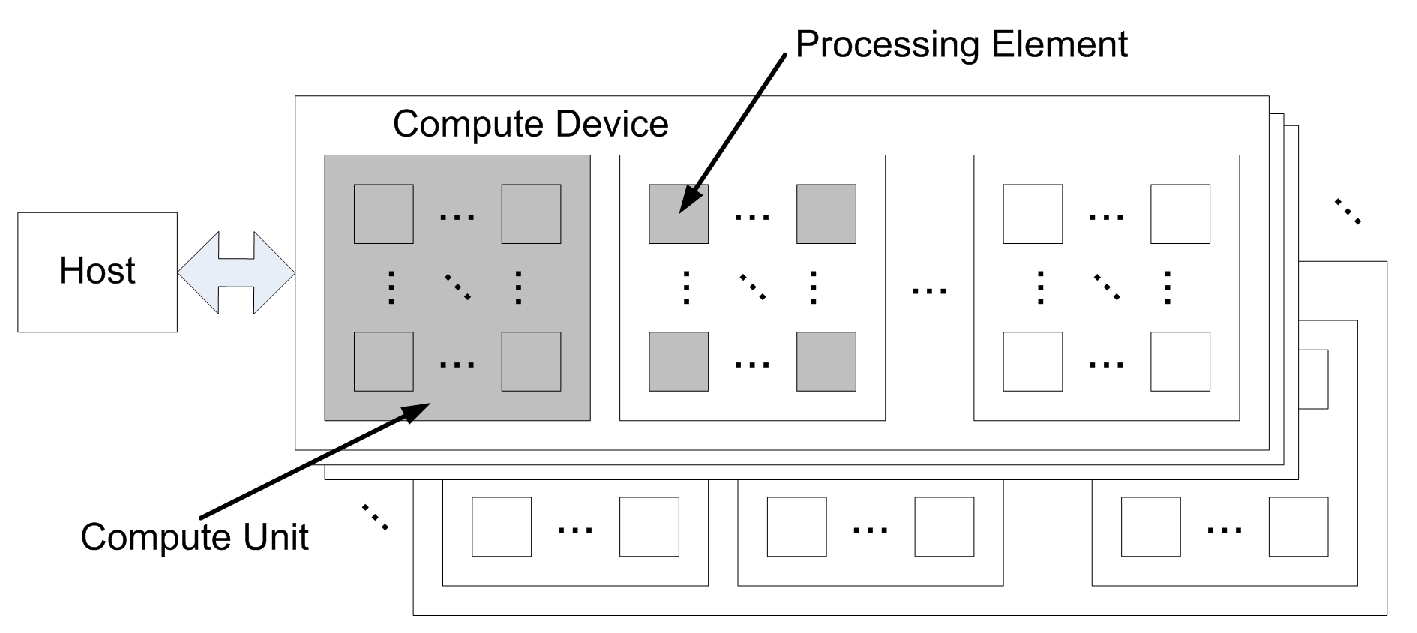
\epsfig{file=./openclfigure2small.eps,width=10cm}}
\caption{GPUs can be seen as SIMD multi-core processors. Internally the GPU contains a number of small processors that are used to perform calculations. Depending on the GPU, the number of threads that can be executed in parallel is in the order of hundreds to thousands.}
\label{figure:openclfigure2small}
\end{figure}

GPUs are specialized stream processors, initially useful for rendering graphics applications. Typically, a GPU is able to perform graphics manipulations at a much higher speed than a general purpose CPU, since the graphics processor is specifically designed to handle certain primitive operations which occur frequently in graphics applications. Internally, the GPU contains a number of small processors that are used to perform calculations. 
Depending on the power of a GPU, the number of threads that can be executed in parallel on such devices is currently in the order of hundreds to thousands and it is expected to multiply in a few years. Nowadays, developers can write (easily) their own high-level programs on GPU. Due to the wide availability, programmability, and high-performance of these consumer-level GPUs, they are cost-effective for, not just game playing, but also scientific computing.
Now, GPUs are exposed to the programmer as a set of general-purpose shared-memory Single Instruction Multiple Data (SIMD) multi-core processors (see Figure \ref{figure:openclfigure2small}). This makes these architectures well suited to run large computational problems, such as those from bioinformatic area. 

Then, the goal of this article is to review the use of GPUs to solve bioinformatic problems, explaining the general approach to using a GPU and given an overview of currently available software systems.

To this end, the rest of this paper is structured as follows: Section \ref{sec:parall_and_GPUs} presents GPUs as highly parallel devices architectures.
Section \ref{sec:programming} gives a background on the different higher level programming languages used to profit GPUs. Finally, Section \ref{sec:bioinfor_apps} reviews different bioinspired approaches using GPUs, followed by a brief conclusion (Section \ref{sec:conclusions}).

%%%%%%%%%%%%%%%%%%%%%%%%%%%%%%%%%%%%%%%%%%%%%%%%%%%%%%%%%%%%%%%%%%%%%%%%%%%%%%%
\section{Throughput, parallelism and GPUs}
\label{sec:parall_and_GPUs}
%%%%%%%%%%%%%%%%%%%%%%%%%%%%%%%%%%%%%%%%%%%%%%%%%%%%%%%%%%%%%%%%%%%%%%%%%%%%%%%

Moore's Law describes a long-term trend in the history of computing hardware: the number of transistors that can be placed inexpensively on an integrated circuit has doubled approximately every two years. The trend has continued for more than half a century and is not expected to stop, theoretically until not too many years above 2015. On 2005 Gordon Moore stated in an interview that his law cannot be sustained indefinitely because transistors would eventually reach the limits of miniaturization at atomic levels. Maybe it is time for Koomey's Law \cite{10.1109/MAHC.2010.28} to replace Moore's Law. Koomey says that energy efficiency is doubled every 18 months. For fixed computing load, the amount of battery you need will fall by a factor of two every year and a half.

Parallel computation has recently become necessary to take full advantage of the gains allowed by Moore's law. For years, processor makers consistently delivered increases in clock rates and instruction-level parallelism, so that single-threaded code is executed faster on newer processors with no modification. Now, to manage CPU power dissipation, processor makers favor multi-core chip designs, and software has to be written in a multi-threaded or multi-process manner to take full advantage of the hardware.

Graphics processors have rapidly matured over the last years, leaving behind their roots as fixed function accelerators, and growing into almost general purpose computational devices for highly parallel workloads. Some of the earliest academic work about GPUs as computational devices date back to University of Washington in 2002 \cite{Thompson:2002:UMG:774861.774894} and Stanford in 2004 \cite{Buck:2004:BGS:1015706.1015800}. 

GPUs are similar to multi-core CPUs but with two main differences (see Figure \ref{figure:captura2paperCEC}). CPUs are made for speedup and GPUs for throughput. CPUs try to improve the execution of a single instruction stream while GPUs take the opposite route obtaining benefits from massively threaded streams of instructions and/or data. The second difference is how threads are scheduled. The operating system schedule threads over different cores of a CPU in a preemptive fashion. GPUs have dedicated hardware for the cooperative scheduling of threads.

\begin{figure}[ht]
\centerline{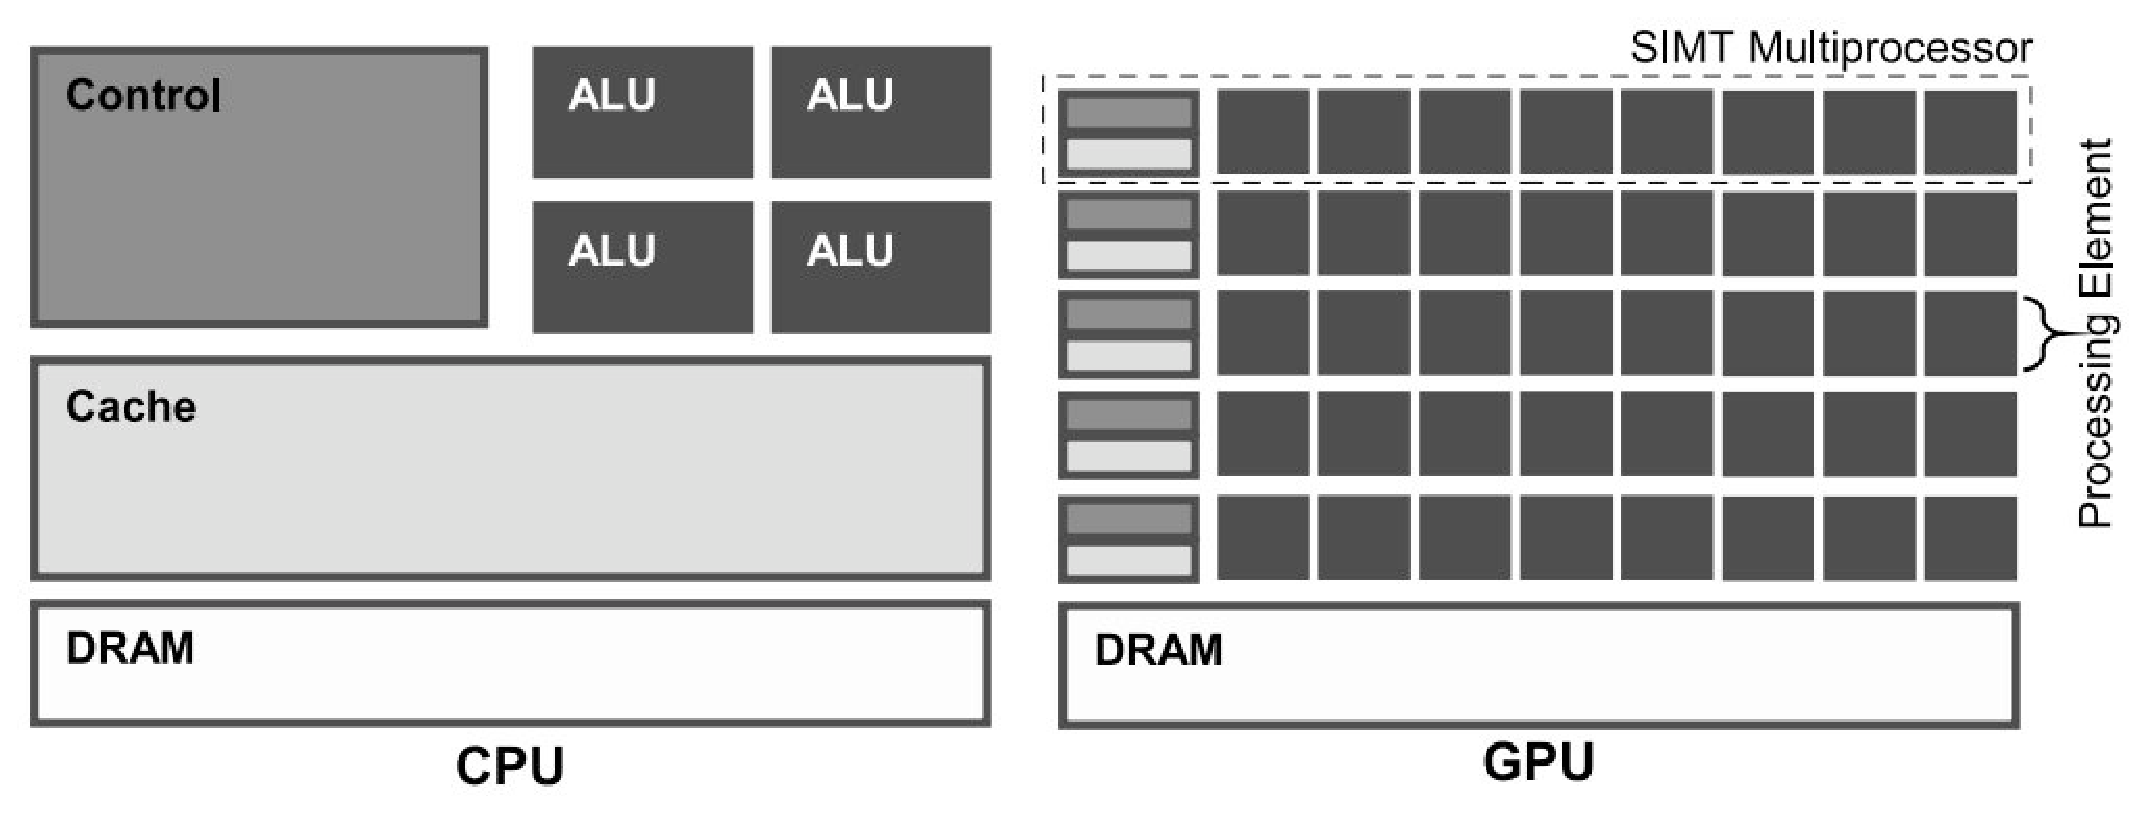
\epsfig{file=captura2paperCEC.eps,width=10cm}}
\caption{CPU-GPU blocks arrangement: The GPU architecture devotes more transistors to data processing.}
\label{figure:captura2paperCEC}
\end{figure}

Physically GPUs used to be huge in comparison with CPUs, see Table \ref{fig:cpugpu}. Latest microprocessors from the two main vendors, AMD \cite{amd} and Intel \cite{intel}, are over 1 billion transistors. Latest GPUs from AMD and NVIDIA \cite{nvidia} are over 4 billion transistors. CPUs draw 130W at most, a limit established by the cost of commodity heat sink and fan. GPUs have increase power consumption and currently are in the neighborhood of 300W. This can be possible with the use of exotic cooling solutions. CPUs are built with the finest technology, read best lithography, while GPUs are made with budget in mind in more common and older processes.

No standard terminology can be found in the world of graphics hardware.
Every company have a very different set of words to refer to the same underlying objects and principles. Many authors try to alleviate this lack of standard terms calling `shader core' to an Intel Execution Unit (EU), an AMD Single Instruction Multiple Data (SIMD) or an NVIDIA Streaming Multiprocessors (SM). Any of these refer to a single processor core inside of the GPU that can fetch, decode, issue and execute several instructions. The shader core is composed of several execution units' or EU that can execute an individual vector operation equivalent to an Advanced Vector Extensions (AVX) or Streaming SIMD Extensions (SSE) instruction. AMD call this kind of EU streaming processor (SP), while NVIDIA uses the term CUDA core. Table \ref{fig:cpugpu} compares several existing CPUs, GPUs and Accelerated Processing Units (APUs), taking into account these terms and their meaning.

\begin{table}[h]
\tbl{CPU, GPU and APU comparison of the best professional and commodity desktop hardware available nowadays. A slash is used in APUs to separate CPU/GPU parts.\label{fig:cpugpu}}
{
\begin{tabular}{|c|c|c|c|c|c|c|c|c|}
\hline
manufacturer           & estimated     & die          & (shader)      & clock rate & memory       & GFLOPS          & TDP & approx. \\
\&                     & transistors   & area         & cores         & (GHz)      & bandwidth    & (single         &     & price   \\
model                  & (billions)    & ($mm^2$)     & CPU[/GPU]     & CPU[/GPU]  & (GB/s)       & precision)      & (W) & (\$)    \\
\hline
\hline
AMD Opteron 6386 SE    & 2.4           & 630          & 16            & 3.5        & 75           & 332.8           & 140 & 1392    \\
\hline
Intel Xeon E5-2697v2   & 2.27          & 434          & 12            & 2.7        & 77           & 536.3           & 130 & 2614    \\
\hline
\hline
AMD A10-7850K          & 2.41          & 245          & 4/512         & 3.7/0.72   & 15           & 856             & 95  & 173     \\
\hline
Intel Core i7 4770K    & 1.4           & 177          & 4/20          & 3.9/1.25   & 21.33        & 177             & 84  & 339     \\
\hline
\hline
AMD Radeon R9 290X     & 6.2           & 438          & 2816          & 1.0        & 320          & 4840            & 275 & 549     \\
\hline
NVIDIA GeForce GTX 780 Ti & 7.1        & 561          & 2880          & 0.87       & 336          & 4000            & 250 & 1000    \\
\hline
\hline
AMD Radeon HD 7990     & $2\times4.3$  & $2\times352$ & $2\times2048$ & 0.95       & $2\times288$ & 8200            & 375 & 700     \\
\hline
NVIDIA GeForce GTX 790 & $2\times7.1$  & $2\times561$ & $2\times2496$ & 0.8        & $2\times336$ & 8000            & 350 & 1000    \\
\hline
\hline
AMD FirePro S10000     & $2\times4.3$  & $2\times352$ & $2\times1792$ & 0.825      & $2\times240$ & $2\times2956.8$ & 375 & 3000    \\
\hline
NVIDIA QUADRO K6000    & 7.1           & 561          & 2880          & 0.9        & 288          & 3950            & 225 & 3000    \\
\hline
\hline
NVIDIA Tesla K40       & 7.1           & 561          & 2886          & 0.745      & 288          & 5364            & 235 & 4000    \\
\hline
Intel Xeon Phi 5100P   & 5             & 600          & 60            & 1.053      & 320          & 2020            & 225 & 2200    \\
\hline
%\hline
%NVIDIA Tegra K1 (32b)  & 5             & $\approx395$ & 4/192         & 2.3/0.95   & 17           & 5600            & 5   & ?       \\
%\hline
%NVIDIA Tegra K1 (64b)  & 5             & $\approx395$ & 2/192         & 2.5/0.95   & 17           & 5600            & 5   & ?       \\
%\hline

\end{tabular}
}
\end{table}

Nowadays NVIDIA has the best single chip GPU discrete card with superior performance in some workloads and AMD the best card with two GPU chips. Both makers takes different compromises in the design of theirs GPUs. AMD has more execution units but its memory hierarchy is weaker. This way software bounded by memory bandwidth or with strong ordering inter-dependencies prefers NVIDIA hardware. On the other side, loads capped by pure ALU execution power use to be faster on AMD hardware.

Traditionally CPUs and GPUs has been separated. Now the trend is to integrate both into a single chip for cost efficiency reasons. Only top models remain as discrete devices. Some of this are top models from Intel's Core i7 or AMD's Opteron 6300 familys. Also best discrete GPUs from NVIDIA and AMD, like consumer GeForce GTX 690 and Radeon HD 7990 and professional line QUADRO K6000 and Radeon FirePro S10000.

Recently, CPU with an integrated GPU have appeared. AMD and Intel have just started selling this kind of combined processor and graphics card. The term Accelerated Processing Unit has been coined for this kind of chips. The architectural names are Llano for AMD and Sandy Bridge for Intel. Many reviews state that AMD's CPU cores are slower than Intel's ones but their GPU is faster. Which combination is better is not an easy question to answer. It must be backed by specific benchmarks, or better, the real application that we want it to run.

Over time the use of GPUs has passed from odd to common in our systems. Actually, several time consuming processes has been parallelized inside our operating systems such as web page rendering. However, the speedup that graphics hardware can bring to us is not free, as each application to be accelerated must be rewritten to take advantage of the GPU.

Figure \ref{fig:gk110}a shows the internals of latest NVIDIA Kepler GK110 architecture. There can be a maximum of 15 SMX units and every one of this has 192 single precision CUDA cores. The six squares on the sides are memory interfaces for a total bus width of 384 bits. It is capable of a maximum bandwidth of 250GB/s connected to GDDR5 memory chips. Figure \ref{fig:gk110}b shows a disclosed SMX unit with its 192 CUDA cores. The maximum theoretical throughput in simple precision is 3950GFLOPS.

\begin{figure}[ht]
\begin{tabular}{cc}
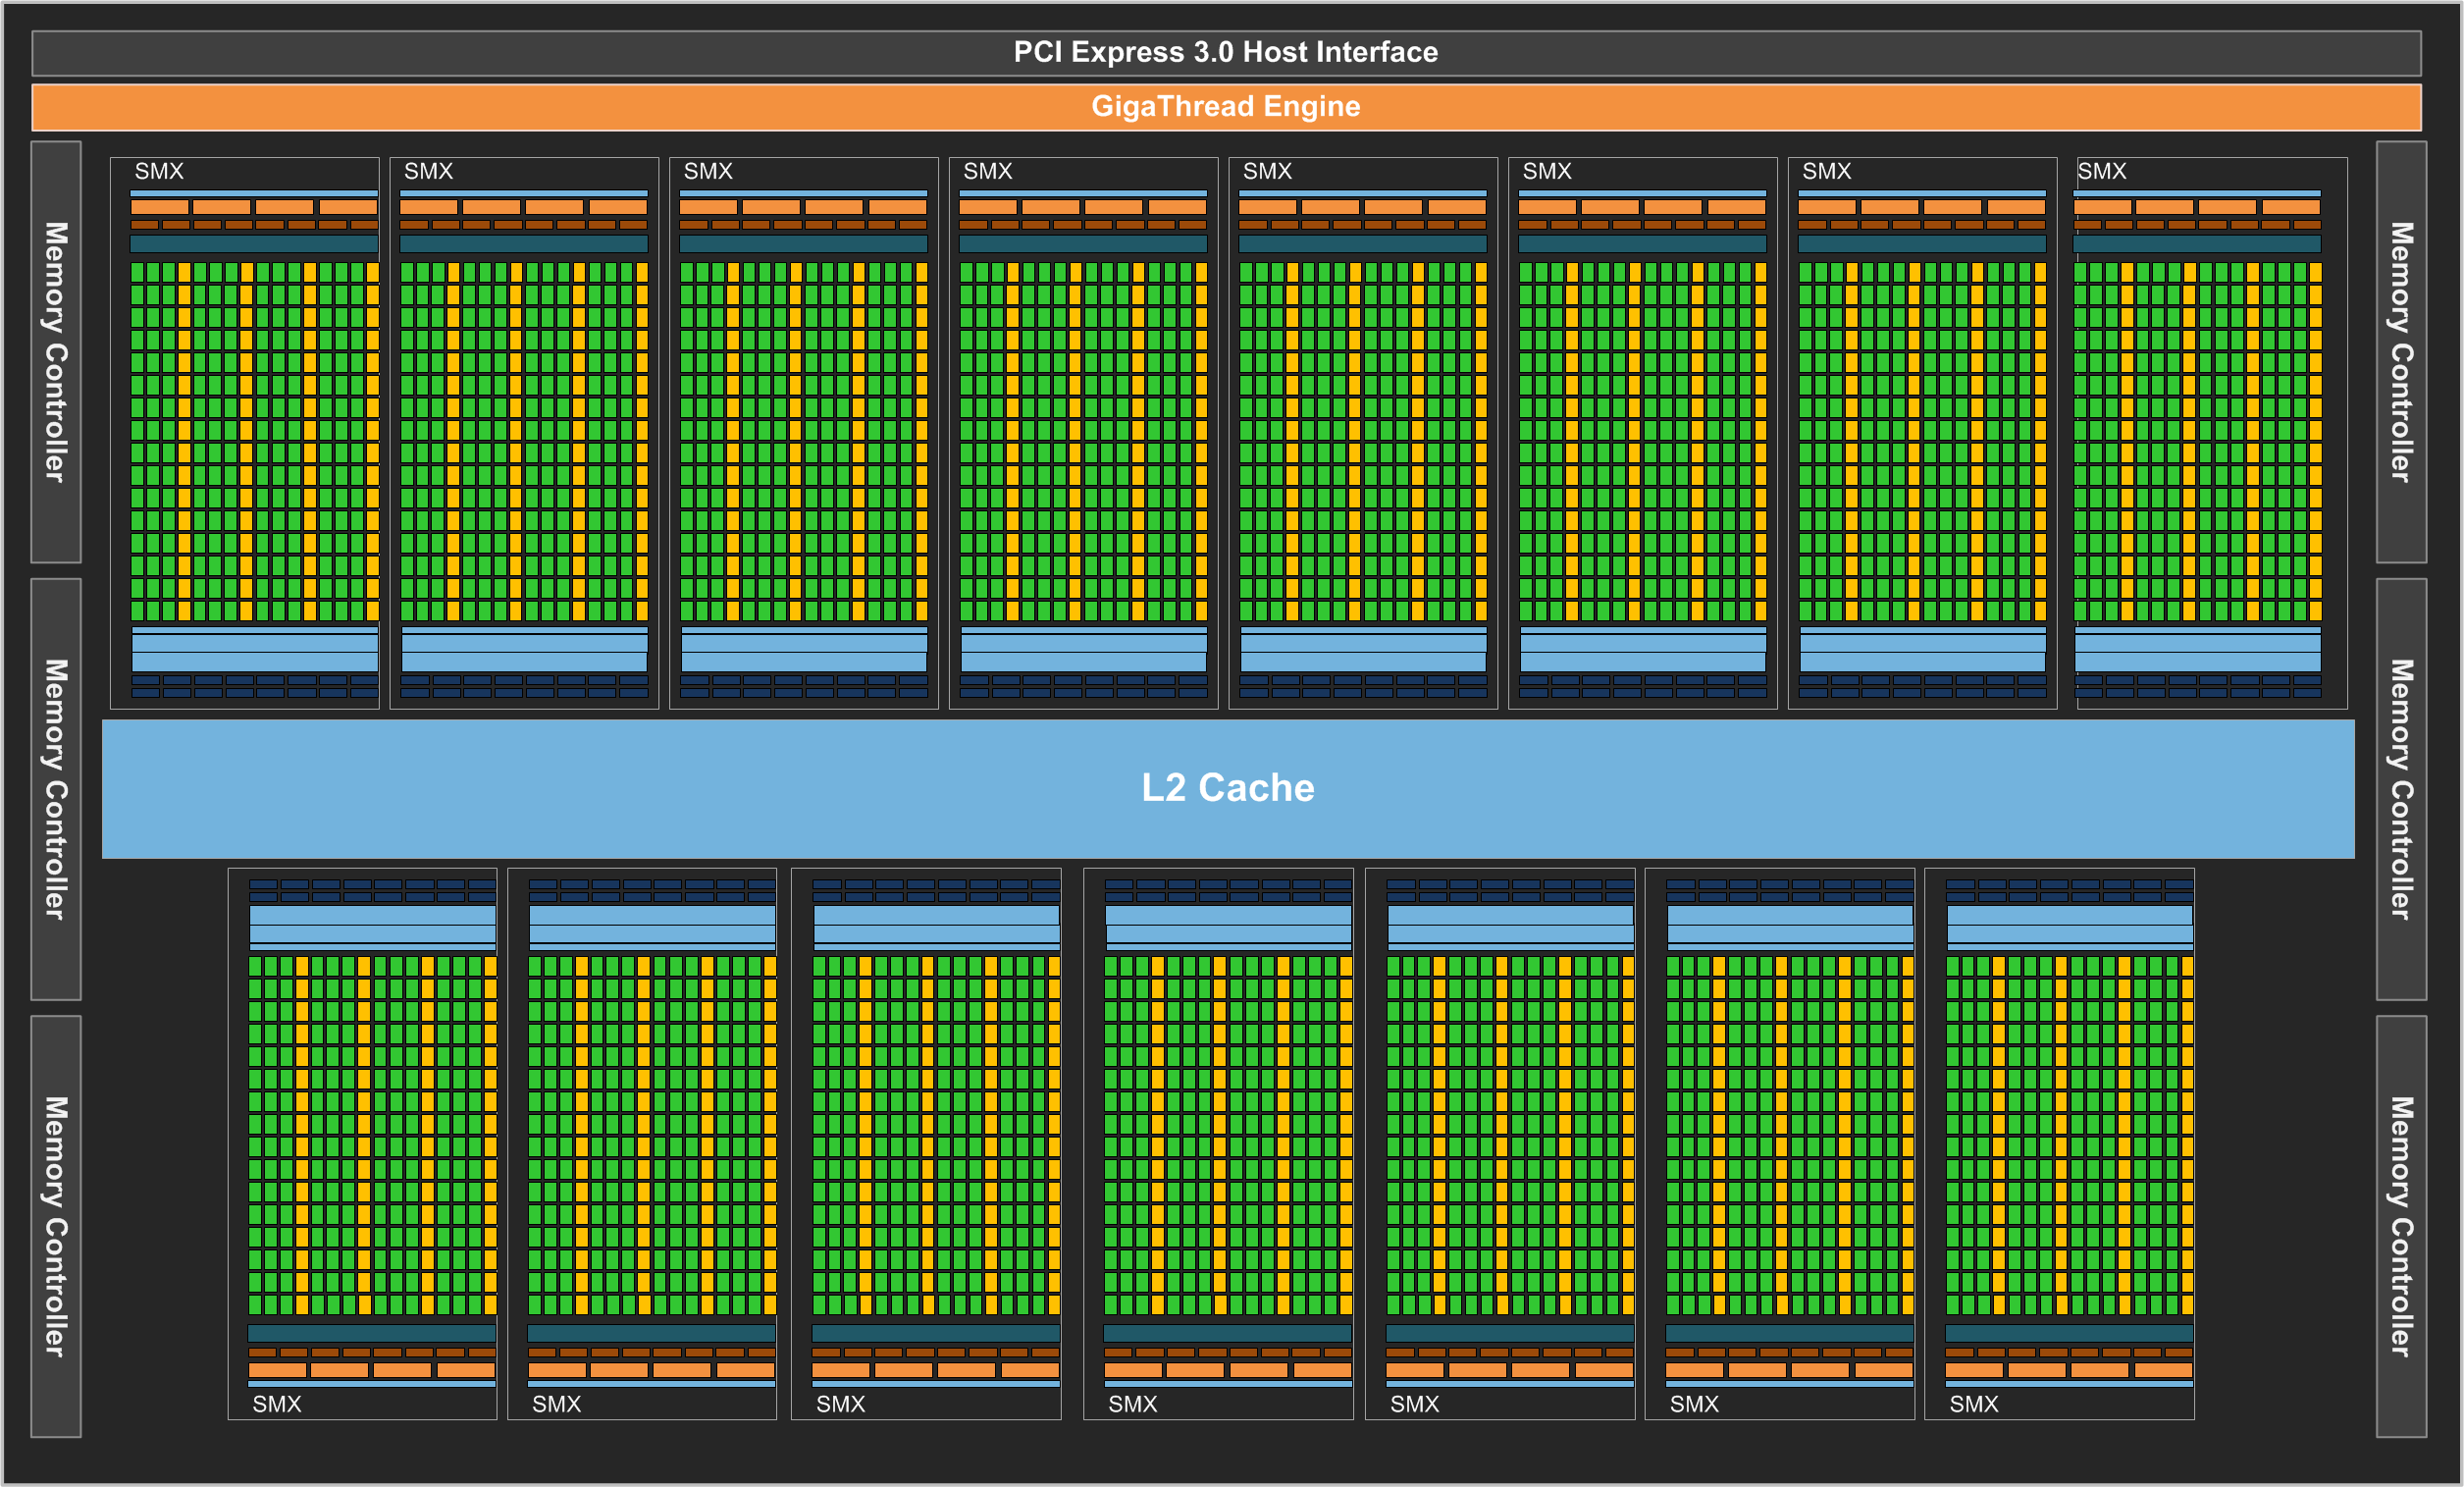
\epsfig{file=./nvidia-gk110.eps,height=5.20cm} & 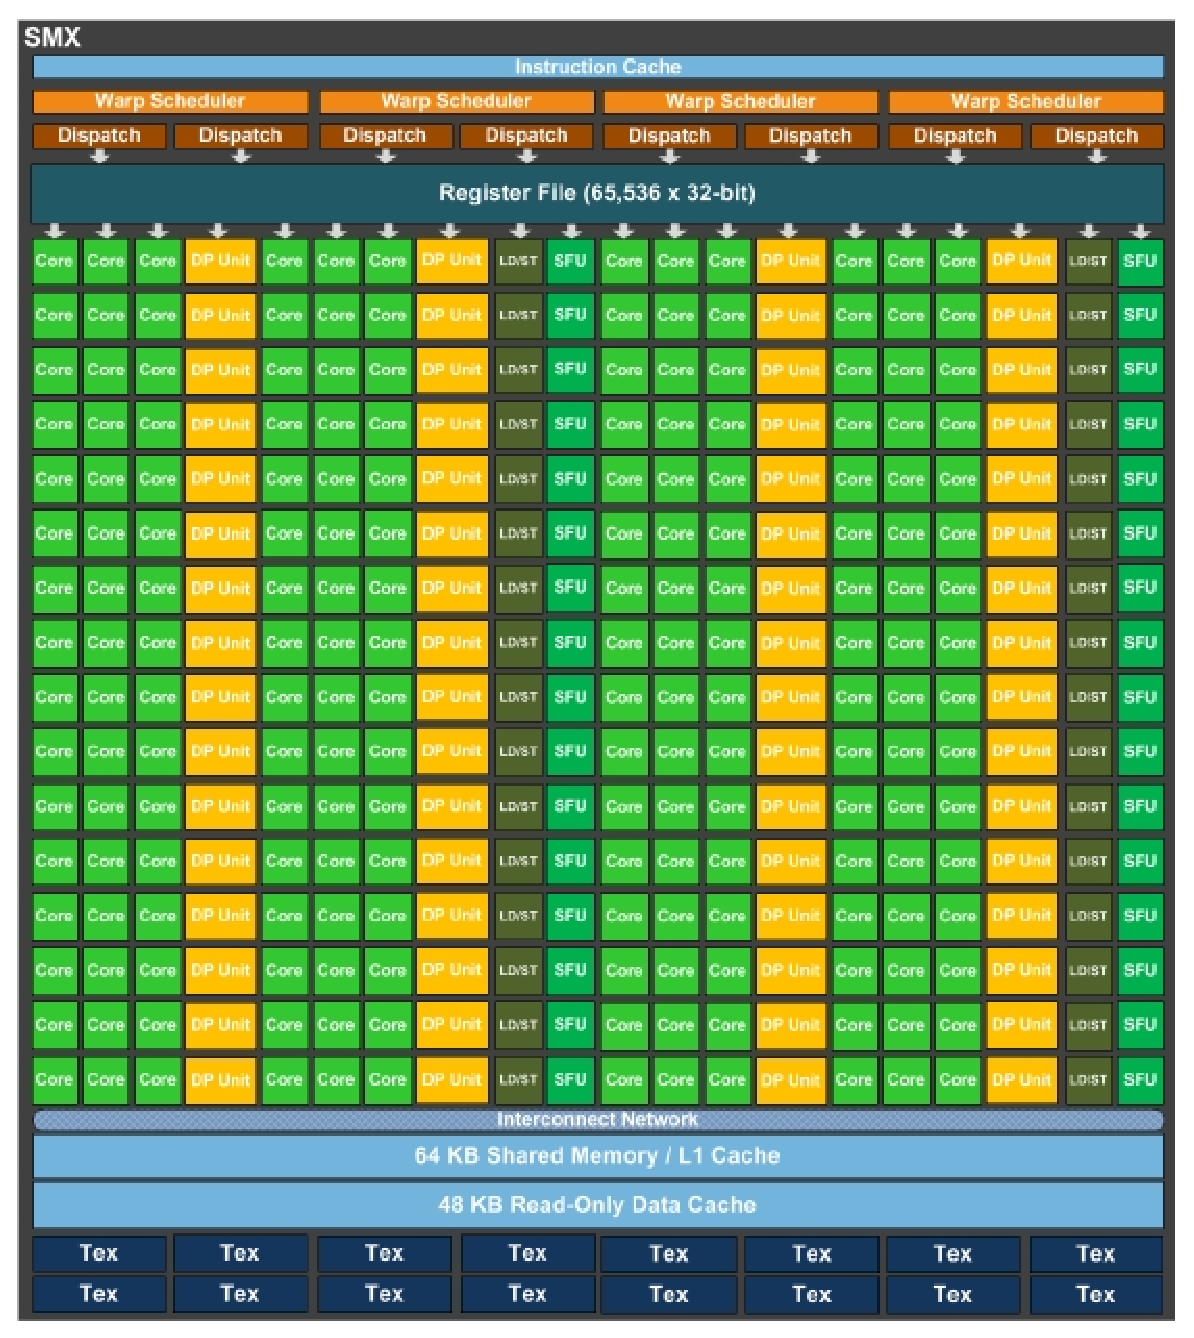
\epsfig{file=./nvidia-smx.eps,height=5.20cm} \\
(a) Block diagram. & (b) SMX unit. \\
\end{tabular}
\caption{NVIDIA Kepler GK110 architecture.}
\label{fig:gk110}
\end{figure}

In the Figure \ref{fig:tahiti}a the newest AMD GPU can be seen. It has an architecture called Graphics Core Next (GCN). Every chip, there are 2, is composed by 28 Compute Units (CU) as AMD call it. Every CU is composed by 4 SIMD vector processors. Every SIMD processor can operate on 16 number simultaneously. This way 1792 instructions can be finalized every clock. Every Tahiti chip has six 64-bit dual channel memory controllers (gray rectangles at the bottom of Figure \ref{fig:tahiti}b) connected to 2 GDDR5 memory channels for a total bandwidth of 240GB/s. The maximum theoretical throughput in simple precision for this design is 2956GFLOPS.

\begin{figure}[ht]
\begin{tabular}{cc}
\epsfig{file=./amd-tahiti.eps,width=6.5cm} & 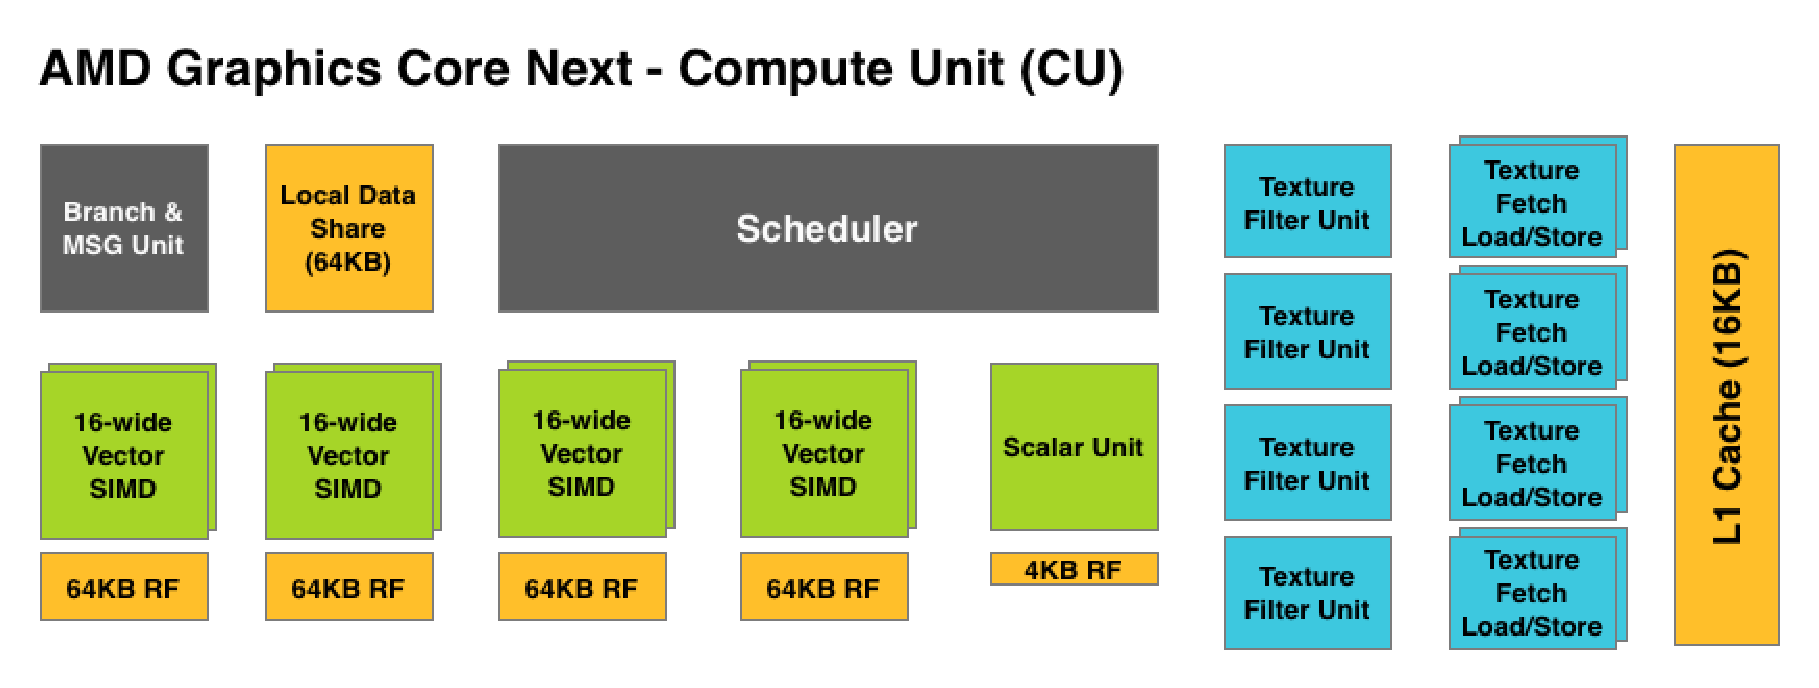
\epsfig{file=./amd-gcn-cu-2.eps,width=6.5cm} \\
(a) Block diagram. & (b) Compute Unit, a SIMD processor. \\
\end{tabular}
\caption{AMD Graphics Core Next architecture.}
\label{fig:tahiti}
\end{figure}

As CPU makers did some years ago, passing from single core to symmetric multiprocessing system (SMP), and more recently to multi-cores, GPU makers follow the same trend. We can connect more than one graphic card to our computer to improve its GPU capacities or buy a card with 2 graphic chips inside. GPUs are so much powerful than CPUs that even a small cluster of a few GPUs can be faster than classic, and much more expensive, big cluster of processors. First cluster of this kind appear in the scientific literature in 2004 \cite{10.1109/SC.2004.26} with big success. Nowadays, more and more people build small GPU clusters with a couple of mighty graphic cards just to game. Connecting 2, 3 or 4 graphics card is called CrossFire by AMD and Scalable Link Interface (SLI) by NVIDIA.

The information shown in this and next sections is available from the websites of the respective manufacturer: AMD \cite{amd}, Intel \cite{intel} and NVIDIA \cite{nvidia}.

%%%%%%%%%%%%%%%%%%%%%%%%%%%%%%%%%%%%%%%%%%%%%%%%%%%%%%%%%%%%%%%%%%%%%%%%%%%%%%%
\section{GPUs Programming}
\label{sec:programming}
%%%%%%%%%%%%%%%%%%%%%%%%%%%%%%%%%%%%%%%%%%%%%%%%%%%%%%%%%%%%%%%%%%%%%%%%%%%%%%%

%%%%%%%%%%%%%%%%%%%%%%%%%%%%%%%%%%%%%%%%%%%%%%%%%%%%%%%%%%%%%%%%%%%%%%%%%%%%%%%
\subsection{Programming Model}
%%%%%%%%%%%%%%%%%%%%%%%%%%%%%%%%%%%%%%%%%%%%%%%%%%%%%%%%%%%%%%%%%%%%%%%%%%%%%%%

The way GPUs can be exploited is deeply rooted on its hardware. There exists several APIs: every company has a proprietary one tied to their respective products. This way AMD started with Close to Metal and NVIDIA with CUDA. Over time another standard appear, OpenCL \cite{opencl}.

With respect to the programming tools available for developers, most the Application Program Interfaces (APIs) are based on C-like languages, but having some restrictions to improve the parallel execution, such as no recursion or limited pointers. Some of them use the open source compiler LLVM \cite{LLVM} from University of Illinois.

From 2003 the two main GPU developers, ATI an NVIDIA, started selling hardware solutions that need to be programmed with proprietary APIs. Despite previous work, the first widely supported GPUs were DX10 generation GeForce 8 series from NVIDIA, using the more mature CUDA API. On the other hand, the Radeon HD2xxx series from ATI, were programmed with the Close To Metal API. 

Paying attention to operating system vendors, there were efforts in the same direction. Some people at Apple betted on the potential of GPUs and started developing an open API, latter known as OpenCL. In the same time, Microsoft created the DirectCompute API for Windows.

OpenCL aimed to became the OpenGL of heterogeneous computing for parallel applications. It is a cross-platform API with a broad and inclusive approach to parallelism, both in software and in hardware. While explicitly targeting GPUs, it also considers multi-core CPUs and FPGAs. The applications are portable across different hardware platforms, varying performance while keeping functionality and correctness. The first software implementations date back to 2009.

Most companies support OpenCL across their products. Apart from AMD and NVIDIA we can use it on graphic hardware from S3 and VIA. Also IBM has a version of OpenCL for PowerPC and CELL processors. Intel started to offer support from the APU architecture Ivy Bridge and GPUs. Embedded world is also interested in OpenCL. Imagination Technologies offer support for the SGX545 graphics core. As does Samsung with their ARM based microprocessors.

To make life easier for potential users many libraries are appearing. One significant example are STL like extensions for the C++ language. In \cite{doi:10.1137/120903683} we can read a comparison of several modern C++ libraries providing high-level interfaces for programming multi- and many-core architectures on top of CUDA and OpenCL.

%%%%%%%%%%%%%%%%%%%%%%%%%%%%%%%%%%%%%%%%%%%%%%%%%%%%%%%%%%%%%%%%%%%%%%%%%%%%%%%
\subsection{Execution Model}
%%%%%%%%%%%%%%%%%%%%%%%%%%%%%%%%%%%%%%%%%%%%%%%%%%%%%%%%%%%%%%%%%%%%%%%%%%%%%%%

OpenCL, DirectCompute and CUDA are APIs designed for heterogeneous computing with both a host CPU and an optional GPU device. The applications have serial portions, that are executed on the host CPU, and parallel portions, known as \textit{kernels}. The parallel kernels may execute on an OpenCL compatible device (CPU or GPU), but synchronization is enforced between kernels and serial code. OpenCL is distinctly intended to handle both task and data parallel workloads, while CUDA and DirectCompute are primarily focused on data parallelism. 

A kernel applies a single stream of instructions to vast quantities of data that are organized as a 1-3 dimensional array (see Figures \ref{figure:captura1paperCEC} and \ref{figure:grid}). Each piece of data is known as a work-item in OpenCL terminology, and kernels may have hundreds or thousands of work-items. The kernel itself is organized into many work-groups that are relatively limited in size; for example a kernel could have 32K work-items, but 64 work-groups of 512 items each. 

\begin{figure}[ht]
\centerline{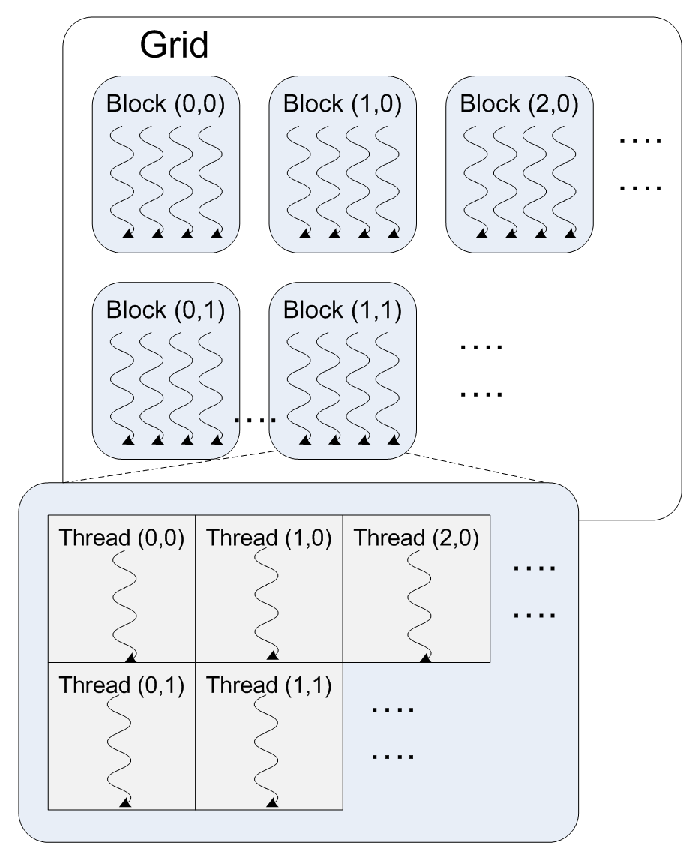
\epsfig{file=./hierarchy.eps,width=7cm}}
\caption{Hierarchy of computing structure in a GPU.}
\label{figure:captura1paperCEC}
\end{figure}

Unlike traditional computation, arbitrary communication within a kernel is strongly limited. However, communication and synchronization is generally allowed locally within a work-group. So work-groups serve two purposes: first, they break up a kernel into manageable chunks, and second, they define a limited scope for communication. 

\begin{figure}[ht]
\centerline{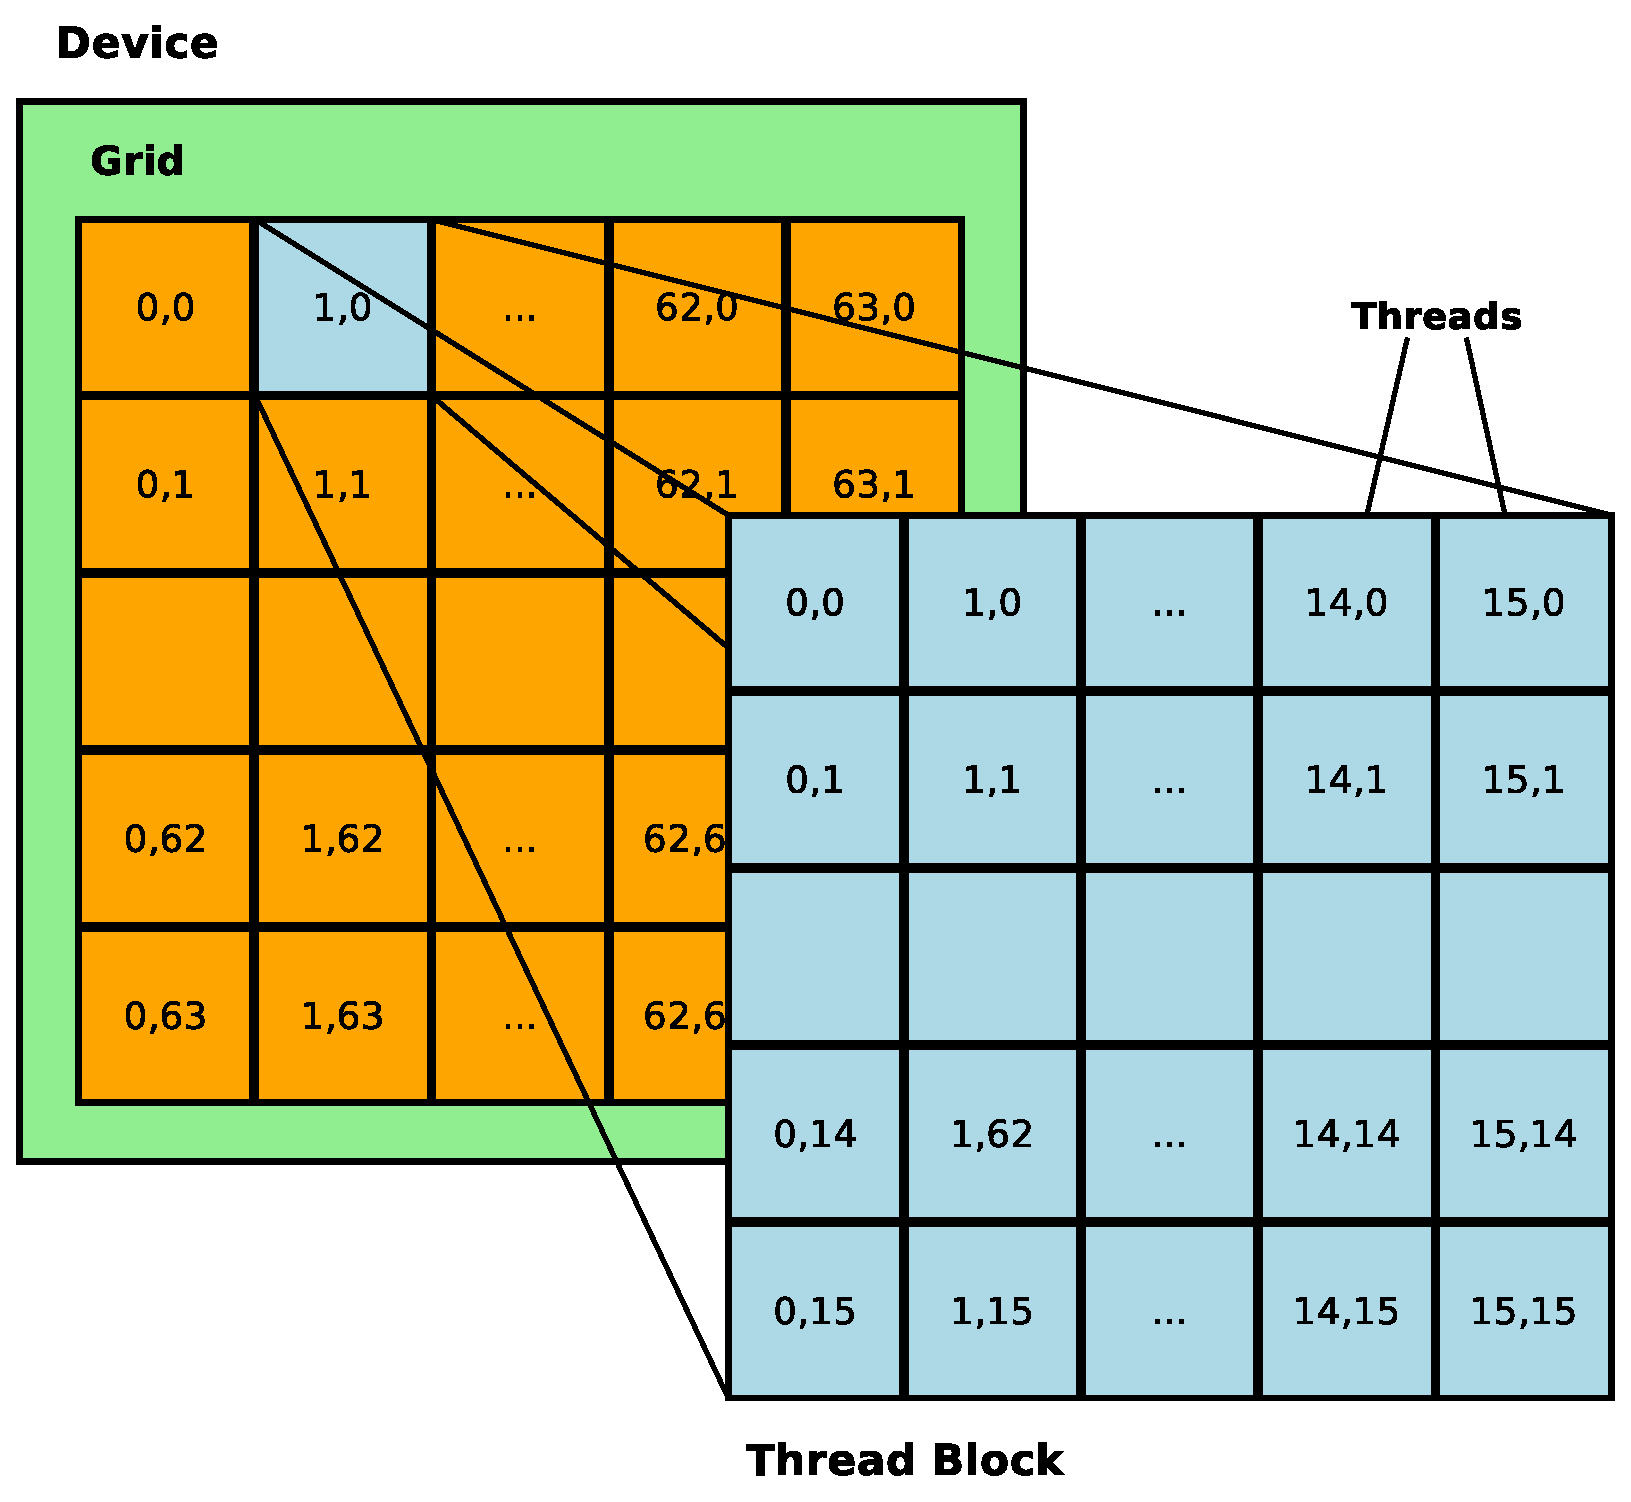
\epsfig{file=grid.eps,width=7cm}}
\caption{Execution model: Each piece of data is a work-item (thread); a kernel has thousands of work-items and is organized into many work-groups (thread blocks); each work-group process many work-items.}
\label{figure:grid}
\end{figure}

%%%%%%%%%%%%%%%%%%%%%%%%%%%%%%%%%%%%%%%%%%%%%%%%%%%%%%%%%%%%%%%%%%%%%%%%%%%%%%%
\subsection{Memory Model}
%%%%%%%%%%%%%%%%%%%%%%%%%%%%%%%%%%%%%%%%%%%%%%%%%%%%%%%%%%%%%%%%%%%%%%%%%%%%%%%

The memory model defines how data is stored and communicated within a device and between the device and the CPU. The memory model can be seen in Figure \ref{figure:memory}. DirectCompute, CUDA and OpenCL share the same four memory types but employ different terminology:

\begin{figure}
\centerline{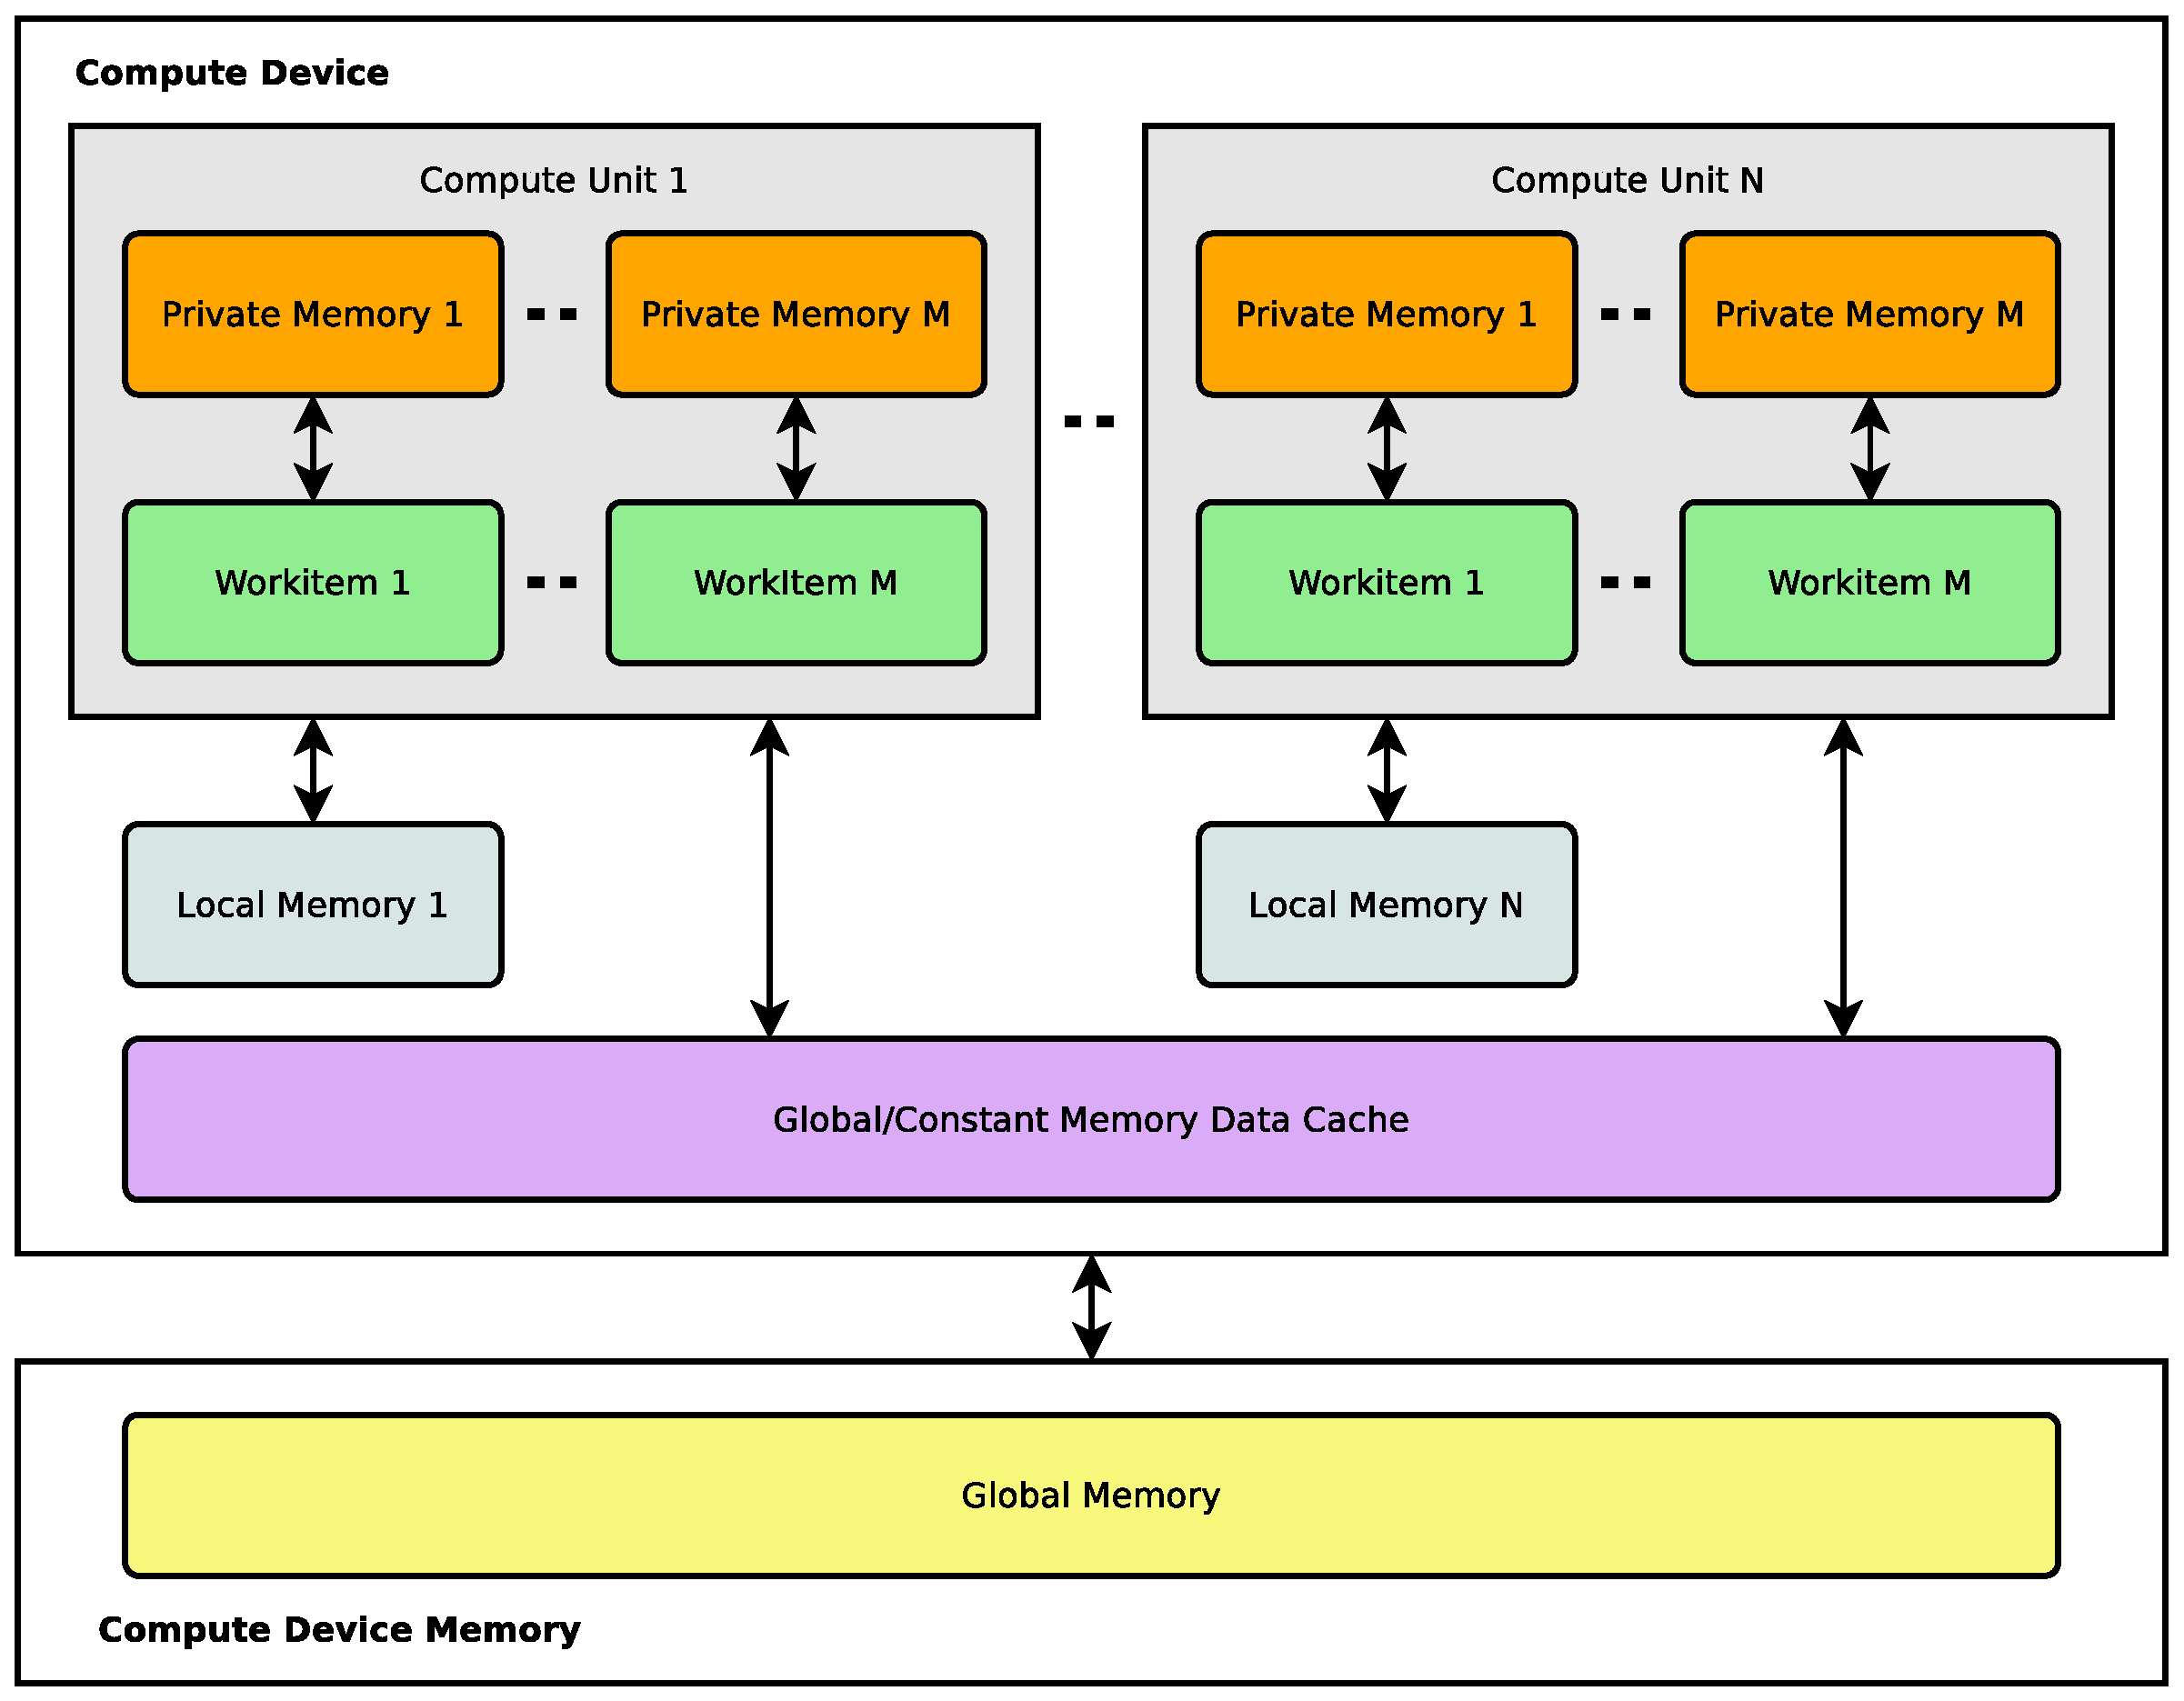
\epsfig{file=memory.eps,width=9cm}}
\caption{Memory model defines how the data is stored and communicated between CPU and GPU. Global memory is RW for both CPU and work-items; constant memory is RW for CPU and RO for work-items; private memory is RW for a single work-item; local memory is RW for a work-group.}
\label{figure:memory}
\end{figure}

\begin{itemize}
\item Global memory: it is available for both read and write access to any work-item and the host CPU.
\item Constant memory: is a read-only region for work-items on the GPU device, but the host CPU has full read and write access. Since the region is read-only, it is freely accessible to any work-item.
\item Private memory: is accessible to a single work-item for reads and writes and inaccessible for the CPU host. The vast majority of computation is done using private memory, thus in many ways it is the most critical term of performance.
\item Local memory: is accessible to a single work-group for reads and writes and is inaccessible for the CPU host. It is intended for shared variables and communication between work-items and is shared between a limited number of work-items.
\end{itemize} 

Unfortunately many times we have to pass data from CPU to GPU before a serious calculation can be done. Also after that, CPU must gather results from the GPU. Too much data passing can ruin speedups so they should be minimized if it can't be avoided at all.

These problem have been with us because current CPUs and GPUs have been designed as separate processing elements and do not work together efficiently. At least until last APUs from AMD. New AMD A7 series uses what the call Heterogeneous System Architecture (HSA). HSA seamlessly shares data between CPU and GPU, without memory copies or cache flushes with minimal dispatch overhead. Both components can share a common memory architecture.

%%%%%%%%%%%%%%%%%%%%%%%%%%%%%%%%%%%%%%%%%%%%%%%%%%%%%%%%%%%%%%%%%%%%%%%%%%%%%%%
\section{Bioinpired Methods on GPUs}
\label{sec:bioinfor_apps}
%%%%%%%%%%%%%%%%%%%%%%%%%%%%%%%%%%%%%%%%%%%%%%%%%%%%%%%%%%%%%%%%%%%%%%%%%%%%%%%

This section reviews different bioinspired approaches included in the bibliography, focusing mainly on Parallel Evolutionary Computation (EC).
Alba et al. \cite{Alba2005book} reviewed and surveyed parallel metaheuristics on EC. They identified the majority of paradigms to be hosting parallel/distributed Evolutionary Algorithms (EAs), according to Flynn's taxonomy, under the Multiple Instruction Multiple Data (MIMD) category. This argument has been fairly valid during the last two decades because the most dominant platform for running parallel/distributed EAs were distributed memory architectures, like clusters, but the fine-grained EAs on massive parallel processors (MPPs) are resurfacing because GPUs architecture gives low cost support for them.

The parallel EAs community has a long legacy with MIMD architectures compared to a very little contribution for SIMD systems. This comes in part due to the dominance of MIMD architectures as compared to SIMD ones.

Alba classifies the main parallel metaheuristic models as follow:
\begin{itemize}
\item Parallel Genetic Algorithms (Cant\'u Paz \cite{Cantu-Paz98asurvey}) %(G. Luque, et al.).
\item Parallel Genetic Programming (F. Fernández, et al.\cite{springerlink:10.1023_A:1021873026259}).
\item Parallel Evolution Strategies (G. Rudolph \cite{Rudolph92parallelapproaches}).
\item Parallel Ant Colony Algorithms (S. Janson, et al. \cite{ParallelAntColony}).
\item Parallel Estimation of Distribution Algorithms (J. Madera, et al. \cite{springerlink:10.1007_3_540_32494_1_7}).
\item Parallel Scatter Search (F. Garcia, et al. \cite{GarciaLopez2003575}).
\item Parallel Variable Neighborhood Search (F. Garc\'ia-l\'opez, et al.\cite{Garcia_lopez_theparallel}).
\item Parallel Simulated Annealing (\cite{Genetic_parallelsimulated}) .
\item Parallel Tabu Search (T. Crainic, et al.\cite{Crainic97towardsa}).
\item Parallel Greedy Randomized Adaptive Search Procedures (M. Resende and C. Ribeiro \cite{Resendeparallelgreedy}).
\item Parallel Hybrid Metaheuristics (C. Cotta, et al. \cite{Cotta05e:parallel}). 
\item Parallel MultiObjective Optimization (A. Nebro, et al. \cite{Nebro07mocell:a}).
\item Parallel Heterogeneous Metaheuristics (F. Luna, et al. \cite{ANL04}). 
\end{itemize}

Nevertheless, when the research community uses GPGPU, all the EC approaches are parallel, so we revise the bibliography taking in mind how an algorithm has been parallelized using GPGPU and, the metaheuristic than the paper deals, is not important for this survey.  For that reason, we focus the rest of the survey with the different ways for implementation of parallel evolutionary algorithms as Zhang and Zhenming propose in \cite{ZhangImplementationMasterSlave}: master-slave model \cite{man-leung-wong-parallel-2005}, fine-grained model \cite{jian_ming_li_efficient_2007}, coarse-grained model \cite{Maitre:2009:CGP:1569901_1570089} \cite{pospichalParallelGeneticAlgorithOnCUDA2010} or hierarchical models  \cite{DBLP:conf/gecco/PospichalMOSJ11} that use two or more of the previous parallel approaches in an hierarchical way. 
 
At the end we have included a subsection for non-standard approaches \cite{DBLP:conf/gecco/PospichalMOSJ11} including  papers which may not be included in any of the previous ones because they mapped the algorithm and the problem they solve in a special way that cannot be considered as fine grained, coarse grained or master-slave ones.

%%%%% Maribel, este último párrafo que viene a continuación yo lo quitaría, si se ha hablado de frameworks for GPGPU en las secciones previas, porque aquí no pega nada. Y si se deja, entonces habría que hablar de CUDA, de OpenCL y de alguna librería más que da soporte para GPGPU como JCUDA desde Java, o PUGACE
 
Most of the evolutionary computation metaheuristics can be used with almost zero effort by using existing frameworks. The most complete and comprehensive review of these frameworks is from Parejo \cite{springerlink:10.1007/s00500-011-0754-8}. It is a comparative study of metaheuristic optimization frameworks. As criteria for comparison, a set of 271 features grouped in 30 characteristics and 6 areas has been selected. These features include the different metaheuristic techniques covered, mechanisms for solution encoding, constraint handling, neighborhood specification, hybridization, parallel and distributed computation, software engineering best practices, documentation and user interface. But this survey does not include frameworks with GPGPU support but only for evolutionary computation metaheuristics. 

%%%%HHHHHHH 
%Maribel, esto es para gustavo. Si se incluye parte de frameworks en la primera parte del artículo, el siguiente párrafo debería ir ahí, sino, aquí la verdad es que tampoco pega nada y habría que quitarlo creo yo.

%%%%%%

PUGACE\cite{5586286} is a framework in CUDA for cellular GAs (cGAs), but only for linear neighborhood structures. The architecture of this framework is presented and experiments with the QAP problem are performed. Fitness evaluation uses a thread for each chromosome. Speedups for several problem instances varies from 15 to 18. The execution platform was a Pentium Dual Core at 2.5Ghz and an nVidia GeForce 98000 GTX+. %FERGU: Aquí no pongo nada porque está dicho que es para cellulars y no hay mucho más que decir...

%%%%%%%%%


%%%%%%%%%%%%%%%%%%%%%%%%%%%%%%%%%%%%%%%%%%%%%%%%%%%%%%%%%%%%%%%%%%%%%%%%%%%%%%%
\subsection{Master-slave Approaches}
\label{sec:masterSlave}
%%%%%%%%%%%%%%%%%%%%%%%%%%%%%%%%%%%%%%%%%%%%%%%%%%%%%%%%%%%%%%%%%%%%%%%%%%%%%%%

Master-slave Evolutionary Algorithms solve problems involving computationally expensive fitness functions, where the master node runs the entire algorithm while the slaves execute the fitness evaluation of the individuals. Using this approach, the evaluation of the fitness function is not sequential, but in parallel, so the master-slave version is more efficient because the evaluations usually are the more expensive portion of the total run time.

%________________________________
% maribel: he reescrito el párrafo siguiente entero, hay que revisarlo bien.
The GPU is responsible of fitness evaluation but it does not get involved with other phases of the algorithm like the crossover, selection or even population ordering for the next generation. In this approach, each generation the individuals are copied to the global memory of the GPU, each single processor gets one or more individuals from global memory and puts them into the shared memory, to decrease global memory overhead. After that, each thread evaluates it or them, and stores the result into the global memory again. The most usual is that each single core evaluates one individual. The programmer has to minimise the number of global memory accesses, as well as to minimise data transfers from CPU to GPU and vice versa. Some additional problems might to be faced, like for example, when the individuals need some data for evaluating, like a distance matrix or a dataset. This additional information might to be copied from CPU to GPU once at the beginning of the algorithm and the threads might to access to this data for evaluation minimising the data transfers from CPU to GPU. So, it must be clear than the more CPU-GPU data transfers passes are needed, the slower the program is.

One of the first proposal for parallel Evolutionary Computation using a GPU was done by Wong et al. \cite{man-leung-wong-parallel-2005}. They  proposed an Evolutionary Programming (EP) without crossover for solving five simple test functions, called Fast Evolutionary Programming (FEP). In this master-slave approach, some actions were executed in the CPU, as the main loop of the algorithm, while evaluation and mutation were run into the GPU device because both steps do not need of external information exchange. In this case, the reproduction step implies interaction among, at least, two individuals so the authors eliminated this step in the algorithm. A maximum speedup of x5.02 was obtained when the population size increases. This is the most common organization in GPU implementations, since no interaction among individuals is required during the evaluation, so this step can be fully parallelized. In this paper the individuals was real-coded and the genomes were mapped into the texture memory. Each GPU thread evaluated one individual and returned its fitness at the end of the parallel step to the CPU for the next evolution cycle step.

A GP method proposed by Harding and Banzhaf \cite{4215552} uses the GPU only for performing the evaluation, while the rest of the steps of the algorithm are run on the CPU. The authors tested real-coded expressions up to 10000 nodes, boolean expressions up to 1500 nodes, and some real world problem where they evaluate expressions up to 10000 nodes. In some cases, the results yielded speedup of thousand times.

Zhang et al. \cite{ZhangImplementationMasterSlave} adapt different EAs to a GPU using CUDA. The authors implemented an hierarchical parallel genetic algorithm using a deme model at the high level, and a master-slave schema at the low level. In this implementation, the CPU initializes the populations and distributes them to thread blocks in shared memory. Then, GPU threads within each block run a GA independently, selection, crossover, mutation and evaluation, and migrates individuals to other thread blocks in its neighborhood. In this case, no speedup results were reported.


Van Luong et al. \cite{5586403} published in 2010 a methodology for mapping the search space onto the GPU memory hierarchy in three levels: the distribution of the search process among the CPU and GPU (1), the mapping of the neighborhood in the GPU threads (2) and the effective usage of the texture memory in the context of hybrid EAs. Experiments to solve the QAP problem with CUDA are presented, where the evolutionary process is performed in the CPU and the generation of the Local Search neighborhood are performed on parallel in the GPU, achieving an acceleration of 14,6 times faster. Hardware used is Core 2 Duo 2,67 Ghz and Nvidia GTX 280. As can be seen this work also shows the benefices of using a conjunction of CPU and GPU, being the GPU used only for intensive calculations. %FERGU: añadida la última frase, para indicar lo que decía el revisor de las ventajas de tener GPU y CPU juntas


There are other papers related with the previous approach, like Tsutsui et al. paper \cite{Tsutsui:2011:GECCO}. This chapter uses a master-slave approach with an Ant Colony Optimization (ACO) algorithm \cite{Dorigo:1999:ACO:329055_329062} with Tabu Search \cite{Glover:1997:TS:549765}. Tsutsui uses an Intel Core i7 965 (3.2 GHz) processor and a single NVIDIA GeForce GTX480 GPU. They compare CPU and GPU implementations with and the results showed that GPU computation with MATA, an efficient method for thread assignment cost which they call Move-Cost Adjusted Thread Assignment, showed a promising speedup compared to computation with CPU.


\cite{Pedemonte:2011:BOG:2001858.2002031} studies the difference of using different representations for binary problems in GPUs evaluating GAs: boolean data type versus packing multiple bits in a non boolean data type. The execution platform was a PC with Quad Core Intel Xeon E5530 processor at 2,4 Ghz and a Tesla C1060 with 240 CUDA cores. The CPU only calculates the initial population and a matrix of random number to be used in crossover and mutation by the GPU. The authors review the problem of the data types when GPGPU is used. Several data types of 8, 16, 32, and 64 bits) are compared in CPU and GPU versions. Results shows that
packing in 32 bits data types achieve speedup values of up to 100 compared with boolean data types, specially when the size of the instances increases. This make sense because the Tesla C1060 are equipped with 32-bit integer ALUs. 
%maribel para Fergu: Te pongo esta referencia aquí arriba porque es del 2011. Creo que esto se puede ampliar más. Ten en cuenta que uno de los principales problemas de las GPUs es que están optimizadas para usar float, entonces ellas almacenan cada dato en un float. Si se empaquetan, pues se está ahorrando espacio de memoria, y supongo que de todo eso hablarán en el paper no! FERGU: completado

Cano et al. \cite{SpeedingTheEvaluationofGPCano:2012} described a massively parallel evaluation model using a Genetic Programming algorithm for evolving rules for a dataset classification. They copied the dataset to the GPU global memory, and evaluated the rules (individuals) for each instance of the dataset in parallel (match kernel). At the end, each successful match was reduced getting each individual fitness (reduction kernel). The implementation, based on CUDA, speeds up the fitness calculation phase and greatly reduce the computation time. Results were compared using one, two and four CPU threads and the combination of one or two GPUs of different features (285 cores for GPUa -NVIDIA GeForce 285 GTX- or 480 cores for GPUb -NVIDIA GeForce 480 GTX-). They test three classification algorithms and the results were not very significant for small dataset, but they improved with large datasets until 820x using two GPUs with 480 cores each one. % Maribel, revisado este también


In \cite{Contreras:2012:UGA:2150467.2150469}ors use a CPU-GPU architecture for stock market trading. The proposed architecture offers the benefices of GPU distribution for stock market researchers, rather for computer architecture experts. The authors used Jacket \cite{jacket:Matlab}, a software platform for the rapid development of general purpose GPU (GPGPU) computing applications within the MATLAB computing environment, C, and C++. However, this framework is not longer available \footnote{\url{http://blog.accelereyes.com/blog/2012/12/12/exciting-updates-from-accelereyes/}}. Steps and guidelines to migrate from CPU code to GPU code are explained, what is a grat contribution, because usually, the authors do not include this information in the papers. The algorithm is run in the CPU, but all  {\em for} loops in selection, evaluation, crossover and mutation are translated to Jacket's {\em gfor} to be parallelized in the GPU. Three different CPU configurations are used for the experiments: Pentium 4, Pentium SU41000 and Intel Core i7-860. The former is also combined with an nVidia 460GTX for GPU experiments. Different population size are also tested. The time is reduced to 65\% in comparison with the CPU version. Other conclusions are obtained: higher speedups are obtained increasing the number of individuals, rather increasing the number of evaluations; and tournament selection reduces time over roulette-wheel selection. %FERGU: Añadido lo de "Other conclusions..." y "The propopsed architecture offers.." Y lo de que Jacket ya no existe (viva el software privativo)
%Maribel: Fergu, pero estos hacen la selección en la CPU o en la GPU? porque si la hacen en la GPU no debería de estar en esta sección. FERGU: no, estos tios paralelizan los "for" de cada sección del algoritmo, lo he aclarado en el texto


%%%%%%%%%%%%%%%%%%%%%%%%%%%%%%%%%%%%%%%%%%%%%%%%%%%%%%%%%%%%%%%%%%%%%%%%%%%%%%%
\subsection{Fine-grained Approaches}
%%%%%%%%%%%%%%%%%%%%%%%%%%%%%%%%%%%%%%%%%%%%%%%%%%%%%%%%%%%%%%%%%%%%%%%%%%%%%%%

Cellular Evolutionary Algorithms (CEAs)or Fine-grained Evolutionary Algorithms have not had as much impact as other types of PEAs. The main reason is that they adapt themselves very well to the especial hardware architecture, with shared memory, but very bad to other distributed memory architectures. On the other hand, parallel distributed memory architectures supply all loosely coupled algorithms and the fine-grained EAs are not included into this category. The main reason behind that is the high cost of building massively parallel architectures which normally attracted fewer researchers to work on fine-grained EAs. A review of the trends in parallel architectures foresees a radical increase in fine-grained EAs face to face other EA categories. This is due to three reasons: 

\begin{itemize}
\item Growing trend of massive number of processors on chip or card. 
\item The high inter-processors speed which is a major factor affecting the efficiency of fine-grained EAs. 
\item The huge low cost of these architectures which attract a wide base of researchers and developers. 
\end{itemize}

For this category of algorithms, each individual is a parent at the beginning of the algorithm and it look for the second parent by selection in a neighborhood. As a result CEAs provide automatic niching effect, avoiding an early convergence. 

Researchers implement fine-grained algorithm using GPGPU making each scalar processor (SP) evolves an 
individual. The individual interacts with other SPs that belongs to the same Streaming Multiprocessor (SM) to perform the basic operations of the algorithm like crossover or mutation. In this approach most of the algorithm is run within the GPU and not only the evaluation phase like in previous section (\ref{sec:masterSlave}). The GPU architecture assist the neighborhoods emerge since each group of SMs have a shared memory Where SPs access without penalty. The exchange of information between each individual through this shared memory is inexpensive. However, programmers have to be careful with the information exchange between individuals in different SMs. 

The second problem of this approach is the random number generator. The CPU generates random numbers without any problem, but the GPU is not designed for this task. So researchers have to think about this problem. Usually the algorithm's implementation generate at the beginning a big set of random numbers and they are copied to the GPU as a list. After that, the GPU uses the random list as it need and when it need. This approach saves time for random generation but the list of random numbers have to be limited by a size. Moreover, all SPs could use the random numbers, so the list has to be available for every thread. 


Yu et al. \cite{yu-parallel-2005} implemented the first real cellular EA using GPU, for solving the Colville \cite{Ng:2005:DFF:1064290.1064296} problem in 2005. They place the population in a toroidal 2D grid and use the classical Von Newmann neighborhood structure with five cells. They store chromosomes and their fitness values in texture memory on the graphic card, and both, fitness evaluation and genetic operations, are implemented entirely with fragment programs executed in parallel on GPU. Real-coded individuals was represented as a set of 2D texture maps. $BLX-\alpha$ crossover and non-uniform mutation was developed as tiny programs on every pixel at each step in a SIMD-like fashion. They solved some optimization problems and reached a speedup of x15 with a population of 512x512 individuals. They store a set of random numbers at the beginning of the evolution process to solve the random number generation problem when using GPU processors. 

In 2006, Wong et al. \cite{man-leung-wong-parallel-2006} proposed a parallel hybrid GA (HGA) where the whole evolutionary process is run on the GPU, and only the random number generation is done in CPU because GPU does not include random numbers generation. Each individual is set to each GPU thread, and each one selects probabilistically an individual in its neighborhood to mate with. Just one offspring individual is generated each time, and it replaces the old one in that GPU thread. The authors compare their implementation with a standard GA run in a CPU and the FEP \cite{man-leung-wong-parallel-2005} algorithm. Using a new pseudo-deterministic selection method, the amount of random numbers transferred from the CPU is reduced. HGA reaches speedup of 5.30 when compared against the sequential version. In 2009 Wong et al. \cite{wong-implementation-2009} provide implementation details for fine-grained evolutionary algorithms.  

Luo et al. \cite{zhongwen-luo-cellular-2006} implemented a cellular algorithm on GPU to solve three different satisfiability problems (SAT) 
% Antonio - Poner qué significan las siglas SAT
using a greedy local search (GSAT) \cite{Selman93domain-independentextensions} and a cellular GA (cGA). 
They saved local minimums using a random walk strategy, jumping to other search space location. 
The cellular GA adopts a 2D toroidal grid, using the Moore neighborhood, stored on texture GPU memory. This implementation generates the random numbers in the GPU (using a generated seed on the CPU at the beginning of the process). They carried out the experiments using two GSAT implementations, CGSAT (with crossover and without mutation) and PGSAT (without crossover and with mutation) running them on CPU and GPU with different population sizes. A great time reduction was reached using the GPU parallelization approach (from 95ms to 18 ms for CGSAT and from 464ms to 77 ms for PGSAT).

Li et al. \cite{jian_ming_li_efficient_2007} proposed a cellular algorithm on GPU for solving some common approximation functions. The authors reported experiments using big populations (up to 10000 individuals) reaching speedups of x73.6 for some implementations. The novelty of this paper is the bit dataset because it is not easy to deal with bit datasets using a GPU due to the memory size restrictions. The GPUs does not support binary operations, but in this paper the authors dealt with binary individuals of 24 bits  and simulated bit-operator by judging each bit of a binary value is 1 or 0. They faced a general problem for all GPGPU community with bit operations. They proposed to use random-textures for random numbers generation, but the random numbers were generated on CPU previously. 

In \cite{Li:2009:PIA:1726585.1726930} the authors proposed an Fine-grained parallel immune algorithm
 (FGIA) which is an Artificial Immune System combined with evolutionary algorithm to generate several optimization algorithms. They solve three no very large instances of Travel Salesman problem (TSP) using a fine fine-grained parallel algorithm with CUDA C. The paper enlarges the population size of FGIA and maintains better population diversity. In conclusions, they included a sub-linear relation between the population size and the execution time, which made the proposal very useful for solving difficult problems that require huge population sizes.

%____________________________________

Alba et al. \cite{springerlink:10.1007978-3-642-12538-619} use CUDA and store individuals and their fitness values in the GPU global memory. Both, fitness evaluation and genetic operators, are run on GPU (no CPU is used). 
They use a pseudo random number generator provided by the SDK of CUDA named Merseinne Twister. Their experiments include some general discrete and continuous optimization problems, and they compare physical efficiency and numerical efficacy with respect to CPU implementation. 

In \cite{PSO-GPU_Mussi} L. Mussi propose a Particle Swarm Optimization (PSO) approach, where a fine-grained model was implemented by omitting the synchronization step, the main constraint for profiting the parallelization power of GPUs in classical metaheuristics. CUDA threads were considered as processing elements for every particle independently. The experiments compared this implementation with a synchronous one, on a GeForce GTX260AMP and a GeForce GTS450 solving different hard synthetic functions problems. The speed-ups factors in the comparison with the sequential approach are up to 200 using the GTS card for the 100 dimensions Rastrigin problem, considering the asynchronous approach, and around 30 for the synchronous implementation, to cite one instance. In average, the first method doubled the later with respect to this factor.

%%%%%%%%%%%%%%%%%%%%%%%%%%%%%%%%%%%%%%%%%%%%%%%%%%%%%%%%%%%%%%%%%%%%%%%%%%%%%%%
\subsection{Coarse-grained Approaches (island model)}
%%%%%%%%%%%%%%%%%%%%%%%%%%%%%%%%%%%%%%%%%%%%%%%%%%%%%%%%%%%%%%%%%%%%%%%%%%%%%%%

Coarse grained algorithms are the most common among parallel EAs. Generally, coarse-grained algorithms require less tightly coupled parallel architectures, as compared to fine-grained. Coarse grained EAs divide the main population into sub-populations (also known as Islands) where the sub-populations evolve concurrently. This basic feature of coarse-grained EAs hits a physical limit of GPUs. 

In order to run a coarse-grained EA using a GPU, several kernels simultaneously are run where each kernel handles a sub-population is not possible. This limitation of GPU would mean the conventional mechanics of coarse-grained EAs would need to be changed if GPU would be used.

With regard to the last topology (fine-grained EAs), one of the first island models on GPU approaches was published on the GPU competition of GECCO 2009 \cite{gecco2009CompetitionPospichal}. It presents some technical details of an island model entirely hard-coded on GPU, with a ring-like topology. Nevertheless, the evolutionary operators implemented on GPU are only specific to the GECCO competition, and the validity of the experiments just works on a small number of problems.

Tsutsui et al. \cite{1570355} propose run a coarse-grained GA on GPU to solve the QAP problem using CUDA. This is one of the hardest optimization problems in permutation domains. 
Their model generates the initial population on CPU and copied it to the GPU VRAM; then, each subpopulation in a GPU (NVIDIA GeForce GTX285) is evolved. At some generations, individuals in subpopulations are shuffled via the GPU VRAM. 
Results showed a speedup from x3 to x12 (using eight QAP instances), compared to the Intel i7 965 processor. 

The model by Luong et al. \cite{LUONG:2010:INRIA-00520464:1} is based on a re-design of the island model.
Three different schemes are proposed: The first one implements a coarse-grained EA using a master-slave model to run the evaluation step on GPU. The second one distributes the EA population on GPUs, while the third proposal extends the second one using fast on-chip memory. 
Second and third approaches reduce the CPU/GPU memory latency, although their parameters (number of islands, migration topology, frequency and number of migrants) must be adapted to the GPU features. 
Sequential and parallel implementations are compared, obtaining a speedup of x1757 using the third approach.

Pospichal et al. \cite{pospichalParallelGeneticAlgorithOnCUDA2010,9253} propose a parallel GA with island model running on GPU. The authors map threads to individuals, thus, threads-individuals can be synchronized easily in order to maintain data consistency, and on-chip hardware scheduler can swiftly swap existing islands between multiprocessors to hide memory latency. Fast, shared memory within the multiprocessor is used to maintain populations.
Since the population size is limited to 16KB per island on most GPUs, if the population is larger, slower main memory has to be used. The migration process is based on an asynchronous unidirectional ring that requires an inter-island communication (slower main memory has to be used). The authors report speedups up to 7000 times higher on GPU compared to CPU sequential version of the algorithm.

%%%%%%%%%%%%%%%%%%%%%%%%%%%%%%%%%%%%%%%%%%%%%%%%%%%%%%%%%%%%%%%%%%%%%%%%%%%%%%%
\subsection{Hierarchical Models}
%%%%%%%%%%%%%%%%%%%%%%%%%%%%%%%%%%%%%%%%%%%%%%%%%%%%%%%%%%%%%%%%%%%%%%%%%%%%%%%

The hybrid model simply utilizes two or more of the master-slave, coarse-grained and fine-grained in a hierarchical method. At the higher level, an island model algorithm runs while at the lower level the demes, another name for sub-populations, themselves are running in parallel (fine-grained, master-slave or even another island model with high migration rates). Hybrid models are not the most common in legacy EAs due to:
\begin{itemize}
 \item The need for additional new parameters to account for a more complex topology structure. 
 \item The need for hierarchical parallel architectures to host hybrid algorithms, while such hierarchical parallel architectures are not so common. 
\item The high complexity of programming such models. 
\end{itemize}

Nevertheless, for the GPUs, hybrid EAs are a perfect candidate to exploit the hierarchical memory and flexible block sizing in GPUs by well structured populations. 

The design and implementation of a hybrid EA plus local search to solve MAX-SAT over GPUs was thoroughly discussed in \cite{Munawar:2009:HGA:1666141_1666143}. Manuwar et al. uses a hierarchical algorithm of 2D structured sub-populations arranged as islands in a 2D grid. Therefore, each individual has 4 neighboring individuals (north, south, east and west) and each sub-population has 4 neighboring sub-populations (north, south, east and west). Instead of using a conventional algorithm for migration between the sub-populations, they introduced a new technique that they call diffusion. Diffusion is more suitable for implementation of cGAs based pGA over a GPU. In the proposed implementation, the host processor (CPU) acts as a controller while an NVIDIA Tesla C1060 GPU provides the required computational resources. Configuration, memory allocation and initialization are performed over the host processor. After the initialization stage, data is transferred to the device and the code enters a loop. The loop keeps on repeating until the maximum number of generation criteria is satisfied. Results were collected over a system with NVIDIA Tesla C1060 GPU mounted on a motherboard with Intel Core i7 920@2.67GHz as the host CPU. C1060 have 4GB of device memory, 30 streaming multiprocessors, and the total number of processing cores is 240. The maximum amount of shared memory per block is 16KB and clock rate is 1.30GHz. They compare the results of the algorithms over NVIDIA with optimized for local search, mutation, recombination, selection and diffusion (migration) with different implementations using serial implementation, OpenMP implementation over Intel and over Ultra Spark architectures. The found that the maximum speedup is for larger problems, and it is up to 25x if compared the serial implementation over Intel Core 2 Duo 3.3GHz with the NVIDIA implementation. 

In \cite{fjdiego-vrp} F.J. Diego et al proposed a parallel strategy for solving the Capacitated Vehicle Routing Problem (CVRP) by means of an ACO algorithm. They combined the CPU processing, random number generation and centralized pheromone information dealing, with the GPU parallel capabilities: trails initialization, build solutions, choose the best and pheromone evaporation. The experiments were conducted on a GeForce GTX460 in a Pentium Dual Core 2.7GHz with 2GB RAM, using CUDA. The results showed a speed-up of 12 in the best case.

In \cite{ACO-on-GPU_Develacq} A. Develacq test different parallel strategies for the ACO metaheuristic on a NVIDIA Fermi C2050 GPU, on a four-core Xeon E5640 @2.6 GHz with 24GB RAM. The Max-Min Ant System is considered for solving the Traveling Salesman Problem (TSP) for problem sizes to up to 2100 cities. Authors proposed multi-ant (one colony) and multi-colony approaches implemented with CUDA. They distributed the solutions on the GPU processing elements: an ant per thread, and an ant per block respectively. The common structures, pheromone matrix, distances and candidate lists, are stored in shared memory, meanwhile the CPU is used for a preliminary set of random numbers generation and centralized control tasks. For the multi-colony algorithms, a set of ants is assigned to every processing element. This time, almost the whole algorithm is run in the GPU. They obtained speed-ups of up to 19 in the multi-ant, and up to 8 in the multi-colony approaches, having similar solution quality than the original sequential approach.

Authors of \cite{Cecilia201342} proposed three different techniques for improving the classical ACO algorithms parallelization on GPUs: a data parallelism scheme for tour construction on GPU, a GPU-based pheromone updating stage, and a roulette wheel implementation on GPU, called I-Roulette. They introduced the queen ants, associated with CUDA blocks, and the worker ants, associated to CUDA threads. The experiments were performed on a four-core Intel Xeon E5620 running at 2.4 GHz, with 16GB RAM, and a NVIDIA Tesla C2050 Fermi. The proposed techniques lead to obtain a speed-up factor of up to 20 in comparison with the sequential implementation.


In \cite{5586530} three cellular GA versions are compared: a CPU, a mono-GPU and a multi-GPU version, being the first work in use multi-GPU for cEAs. A 2D grid population is used and divided in two GPUs in the multi version. Selection, recombination, mutation and evaluation are performed in parallel. In the multi GPU case, a thread for each GPU is controlled by a CPU thread and borderline individuals of the sub-populations are exchanged. The
speedup ranges from 8 to 711. However, there is not significantly difference between mono and multi GPU versions, probably due the overhead of the CPU. Hardware used is Intel Quad processor 2.67GHz and Nvidia GeForce GTX 285. %FERGU: añadido que es el primero que trabaja con multigpu


%%%%%%%%%%%%%%%%%%%%%%%%%%%%%%%
%Maribel
%Falta incluir el otros dos artículos de Luong no sé exactamente en qué sección cuyas referencias son \cite{luong:Neighborhood2010} y % \cite{LuongParallelHybridEvolutionaryAlgorithmsOnGPUCEC2010} FERGU: Maribel, ese ya lo he comentado yo con el \cite{5586403} lo quito de tu .bib
%Maribel: Ok, 
%%%%%%%%%%%%%%%%%%%%%%%%%%%%%%%%%%%%%%%


% Maribel, este siguiente no me lo he bajado todavía, pero también hay que ampliarlo. 
Experiments running several instances of Fast Ant System \cite{Taillard:1998:FFA:870509}e best neighbor at each iteration of the search and the Quadratic Assignment Problem \cite{Zhu:2010:0020-7543:1035} are shown. They use an Intel Core i7 930 with NVIDIA GTX 480 or the Intel Xeon E5520 with Tesla C1060. The GPU implementation is 15 times faster than the one running on the CPU.


During 2012, Luong et at. run GPGPU algorithm from metaheuristics implementation point of view. In \cite{luongMetaheuristicsPpsn2012} a guideline to exploit heterogeneous computing resources, including GPU and CPUs, for effective hybrid metaheuristics was proposed. The goal of this paper is not the evaluation of the fitness of some individuals, but the parallelization of metaheuristics which were not inherently parallel, like local search algorithms. Task distribution is clearly defined into the paper,  the CPU manages the whole sequential Local Search process and the GPU is dedicated to the costly part i.e. the parallel generation and evaluation of the neighboring solutions.
Authors mapped the population to the GPU and applied the parallel metaheuristic to each individual using its neighborhood structure taking adventage of blocks of threads, so of the GPU architecture. The parallelization of these metaheuristics generated several different individuals that the GPU evaluated at the same time. The critical issue was to find efficient mappings between a GPU threads and a particular neighbor. Indeed, this step is crucial in the design of new large neighborhood local search algorithms for binary problems since it is clearly identified as the gateway between a GPU process and a candidate neighbor. They reviewed neighborhoods based on a Hamming distance of one, two and three and applied their suggestions to Permuted Perceptron problem \cite{KnudsenPermutedPerceptronProblem1999}. They used a Tabu Search algorithm \cite{TaillardTabySearch1991} using CUDA for each neigborhood with a configuration of Intel Core 2 Duo 2.67GHz with a NVIDIA GTX 280 card. The CUDA implementation increased the number of successful solutions drastically every instance of the problem. Regarding execution time, acceleration factors using GPU are very significant (from $24.2x$ to $25.8x$). 

   




\subsection{Non standard Approaches}

Pospichal et al. in 2011 has addressed several papers related with GPU devices. One of the last is \cite{DBLP:conf/gecco/PospichalMOSJ11} where they proposes to use a GPU device for Grammatical Evolution evolving complete programs in an arbitrary language using variable length binary strings. For this problem, the individual is a program, so it must to be compiled and sent to the GPU for evaluation each generation. But the most time-consuming part of this approach is to sent the individuals to the GPU and no the evaluation itself, so, Pospichal et al. propose to evolve the whole Grammatical Evolution algorithm on the GPU with a special mapping function. They mapped one individual per block of threads and one thread is used for manipulate each individual. They compare the execution time of an Intel Core i7 with NVIDIA GTX 480 using CUDA (CPU implementation with C) an a Java library called GEVA \cite{O'Neill:2008:GGE:1527063.1527066} which is interpreted language (CPU implementation using GEVA).  The authors include results for both implementations (C and GEVA) and one GPU implementation and they compare them with and without overhead for CPU-GPU communication. We include only the results with overhead, because the parallel version need the CPU-GPU communication so the authors might to take care about it. The results of GPU implementation are in average 5.3 speedup than CPU with C implementation which is an expected result. The speedup grows until 102.8 when GPU implementation and CPU implementation with GEVA are analysed but the authors do not include any variance results, so we do not recommend the last result as the most important of the paper. Thus, this paper proposes two levels of parallelism: 1) indi-
viduals are evaluated in parallel (by threads in he same block) and 2) data within individuals (genes, crossover points, mutations, fitness points, etc.) are maintained by parallel access as well (by block of threads).



%%%%%%%%%%%%%%%%%%%%%%%%%%%%%%%%%%%%%%%%%%%%%%%%%%%%%%%%%%%%%%%%%%%%%%%%%%%%%%%
\subsection{Artificial Neural Networks implementations on GPUs}
%%%%%%%%%%%%%%%%%%%%%%%%%%%%%%%%%%%%%%%%%%%%%%%%%%%%%%%%%%%%%%%%%%%%%%%%%%%%%%%

Artificial neural networks attempt to capture the adaptability of biological neurons in a mathematical model for information processing. ANNs are very powerful tools that are highly parallel but also computationally expensive and match well with the GPU computing architecture.  As a workhorse of the computational intelligence field, there exists a high demand for  this acceleration.  As a highly analytic structure, neural networks can be reduced to a series of matrix operations, and thus are easily parallelized, as the GPU is highly optimized to perform these kinds of operations \cite{Meuth2006}.  

Several authors provide tips for ensuring efficient implementation  of algorithms on GPU’s \cite{Oh2004,Luo2005,Martinez2007,Martinez2010}.

Zhongwen uses the GPU to first extract a set of characteristics from image data, then applies a pre-trained MLP to these characteristics for classification \cite{Luo2005}.

Bernhard \cite{BernhardCITA17} proposes a different approach, implementing spiking neural networks for image segmentation.

In general, significant performance gains can be elicited from implementing neural network algorithms on graphics processing units. However, these implementations are difficult to obtain.

Finally, several developers provide libraries and tools to help practitioners to develop ANN applications on GPUs \cite{url2}.

%\begin{figure}[b]
%\sidecaption
%\includegraphics[scale=.65]{figure}
%\caption{If the width of the figure is less than 7.8 cm use the \texttt{sidecapion} command to flush the caption on the left side of the page. If the figure is positioned at the top of the page, align the sidecaption with the top of the figure -- to achieve this you simply need to use the optional argument \texttt{[t]} with the \texttt{sidecaption} command}
%\label{fig:1}
%\end{figure}

%\begin{table}
%\caption{Please write your table caption here}
%\label{tab:1}
%\begin{tabular}{p{2cm}p{2.4cm}p{2cm}p{4.9cm}}
%\hline\noalign{\smallskip}
%Classes & Subclass & Length & Action Mechanism  \\
%\noalign{\smallskip}\svhline\noalign{\smallskip}
%Translation & mRNA$^a$  & 22 (19--25) & Translation repression, mRNA cleavage\\
%Translation & mRNA cleavage & 21 & mRNA cleavage\\
%Translation & mRNA  & 21--22 & mRNA cleavage\\
%Translation & mRNA  & 24--26 & Histone and DNA Modification\\
%\noalign{\smallskip}\hline\noalign{\smallskip}
%\end{tabular}
%$^a$ Table foot note (with superscript)
%\end{table}

%%%%%%%%%%%%%%%%%%%%%%%%%%%%%%%%%%%%%%%%%%%%%%%%%%%%%%%%%%%%%%%%%%%%%%%%%%%%%%%
\section{Conclusions}
\label{sec:conclusions}
%%%%%%%%%%%%%%%%%%%%%%%%%%%%%%%%%%%%%%%%%%%%%%%%%%%%%%%%%%%%%%%%%%%%%%%%%%%%%%%

Bioinspired algorithms have been used in traditional computers and clusters in 
the past decades, but with the actual technological enhancement of computer graphics, a new way to execute this kind of algorithms in GPUs has been open. 

This paper shows a survey of the usage of GPUs to execute bioinspired
algorithms to solve optimization problems. An introduction to different GPU architectures, with the languages and frameworks used in the industry has been presented.

Also, a number of works available in the literature have been explained, with a description of a taxonomy to classify them. Most of the studied algorithms use the GPU for parallel fitness evaluation, but other examples for parallel distribution are being implemented, such as Ant Colony Optimization.

In the most of the cases, extremely higher speedups are attained compared with traditional CPU sequential versions. Several authors agree on the bottlenecks due to synchronization in the CPU parts of the algorithms, so new directions 
about minimize the communication with the CPUs are emerging.

%%%%%%%%%%%%%%%%%%%%%%%%%%%%%%%%%%%%%%%%%%%%%%%%%%%%%%%%%%%%%%%%%%%%%%%%%%%%%%%

\begin{acks}
This work has been supported in part by 
the UGR PR-PP2011-5 project, 
%the Junta de Andaluc\'{\i}a {SIPEsCa} (G-GI3000/IDIF) project,
the P08-TIC-03903 project awarded by the Andalusian Regional Government, 
the FPU Grant 2009-2942 
and 
the TIN2011-28627-C04-02 project.

%The authors are grateful to anonymous referees for their constructive comments and advice about the first version of our chapter.
%The authors are very grateful to the anonymous referees whose comments and suggestions have contributed to improve this chapter.
\end{acks}

%%%%%%%%%%%%%%%%%%%%%%%%%%%%%%%%%%%%%%%%%%%%%%%%%%%%%%%%%%%%%%%%%%%%%%%%%%%%%%%
%\section*{Appendix}
%\addcontentsline{toc}{section}{Appendix}
%%%%%%%%%%%%%%%%%%%%%%%%%%%%%%%%%%%%%%%%%%%%%%%%%%%%%%%%%%%%%%%%%%%%%%%%%%%%%%%

\bibliographystyle{acmsmall} 
\bibliography{antonio,gpus,gustavo,maribel,pablo,todo}

\bigskip

% History dates
\received{Dec-2012}{-}{-}

% Electronic Appendix
%\elecappendix

\end{document}

